\chapter{Binding energy of the $^{86}$Sr$_2$ halo molecule}
\label{ch:chap4}

\section{Probing the ground state potential}
\label{sec:lowE_intro}

Strontium is a nice atom to work with because of the various properties of all of it's isotopes but access to such a variety of properties also comes with it share of complications. The most abundant isotope, 88, has a nearly vanishing scattering length but served as the workhorse for many of our previous stuides and those of other labs. The known scattering properties of strontium are mass scaled from 88 \hl{is this somehow not as good for 86? Also, where are the most up to date scattering lengths for Sr from? - The '10 Fourier paper} but by probing the 86 ground state potential directly we can obtain a more accurate measurement of the 86-86 scattering length.

Additionally, by utilizing the narrow intercombination potential we are able to detune many linewidths from the intermediate state, thereby 

Two-photon photoassociation 

umm, I want to write something about the narrow line letting us probe this but 

As described in previous chapters, two-photon PAS can be used to directly populate low-lying molecular levels. Applying this technique to strontium 86 we can explore a similar regime

conclusion of chapter 4 is that we measured the binding energy more accurately which can be directly related to a more precious value of the scattering length for 86. Also there is a straightforward experiment available to use to attempt to measure the efimov paramter for strontium.

how did we determine the binding energy? how did we measure spectra?

% Start of paper
Weakly bound ground-state dimers are of great interest in ultracold atomic and molecular physics. In the extreme case of a scattering resonance, the least-bound state represents an example of a quantum halo system \cite{jrf04} with spatial extent well into the classically forbidden region. Halo molecules show universality, meaning that molecular properties such as size and binding energy can be parameterized by a single quantity, the $s$-wave scattering length $a$, independent of other details of the atom-pair interaction \cite{kgj06,bha06}. For potentials that asymptote to a van-der-Waals form, an additional parameter, the van der Waals length $l_{\mathrm{vdW}}$, can be introduced for a more accurate description. Efimov trimers also exist in systems near a scattering resonance, influencing dimer and atomic scattering properties and introducing additional universal phenomena \cite{bha07,nen17}. Ultracold halo molecules are often associated with magnetic Feshbach resonances \cite{cgj10}, for which the scattering state and a bound molecular state can be brought near resonance by tuning a magnetic field.

%Weakly bound ground-state dimers are of great interest in ultracold atomic and molecular physics. Measurement of the binding energy precisely determines the associated $s$-wave scattering length ($a$) for free-atom collisions. In the extreme case of a scattering resonance, the least-bound state represents an example of a quantum halo system \cite{jrf04} with spatial extent well into the classically forbidden region. Halo molecules show universality, meaning that molecular properties such as size and binding energy can be parameterized by the single quantity $a$ independent of other details of the atom-pair interaction \cite{kgj06,bha06}. For potentials that asymptote to a van-der-Waals form, an additional parameter, the van der Waals length $l_{\mathrm{vdW}}$ can be introduced for a more accurate description. Efimov trimers also exist in systems near a scattering resonance, influencing dimer and atomic scattering properties and introducing additional universal phenomena \cite{bha07,nen17}.
%Ultracold halo molecules are often associated with magnetic Feshbach resonances \cite{cgj10}, for which the scattering state and a bound molecular state  can be brought near resonance by tuning a magnetic field.

%Here, we perform two-photon photoassociation to a naturally occurring halo molecule state in
%$^{86}$Sr. We accurately determine its binding energy and calculate the scattering length using the universal theory for a weakly bound molecule \cite{gfl93,gao04}.
%perform two-photon photoassociation (PA) \cite{jtl06} to

Here we study the least-bound vibrational level of the X$^1\Sigma_g^+$ electronic ground state of the $^{86}$Sr$_2$ dimer (Fig.\ \ref{PASDiagram}), which is a naturally occurring halo molecule, meaning it exists in the absence of tuning with a magnetic Feshbach resonance. A well-known example of a naturally occurring halo molecule is the $^4$He$_2$ dimer \cite{lmk93,sto94,kgj06}. The least-bound vibrational level of the ground state of $^{40}$Ca$_2$, which was recently studied using similar methods \cite{Pachomow2017a}, is also very close to this regime.


%Most studies of halo molecules have been with states associated with a magnetic Feshbach resonance (refs).
%For halo molecules associated with

There are important differences between halo molecules associated with magnetic Feshbach resonances and the naturally occurring halo molecule in $^{86}$Sr. With magnetic Feshbach resonances, the relevant scattering and bound molecular states lie on different molecular potentials, and single-photon magnetic-dipole transitions can be used to measure molecular binding energies with RF or microwave spectroscopy \cite{cgj10,cju05,thw05b}. Typically, this is done by first forming molecules through magneto-association and then driving bound-free or bound-bound transitions converting the halo molecule into a different state. Other methods include spectroscopy with an oscillating magnetic field \cite{thw05b}, a modulated optically controlled Feshbach resonance \cite{chx15}, and Ramsey-type measurements of atom-molecule oscillation frequencies \cite{ckt03}. It is also possible to efficiently populate halo states with a magnetic-field sweep \cite{grj03} or evaporative cooling \cite{jba03} near a magnetic Feshbach resonance \cite{cgj10}. These are powerful techniques for manipulating quantum gases of alkali metals and other open-shell atoms, for which there are many magnetic Feshbach resonances. Strontium, however, due to its closed-shell electronic structure, lacks magnetic Feshbach resonances in the electronic ground state.


\begin{figure} \label{PASDiagram}
\centerline{
  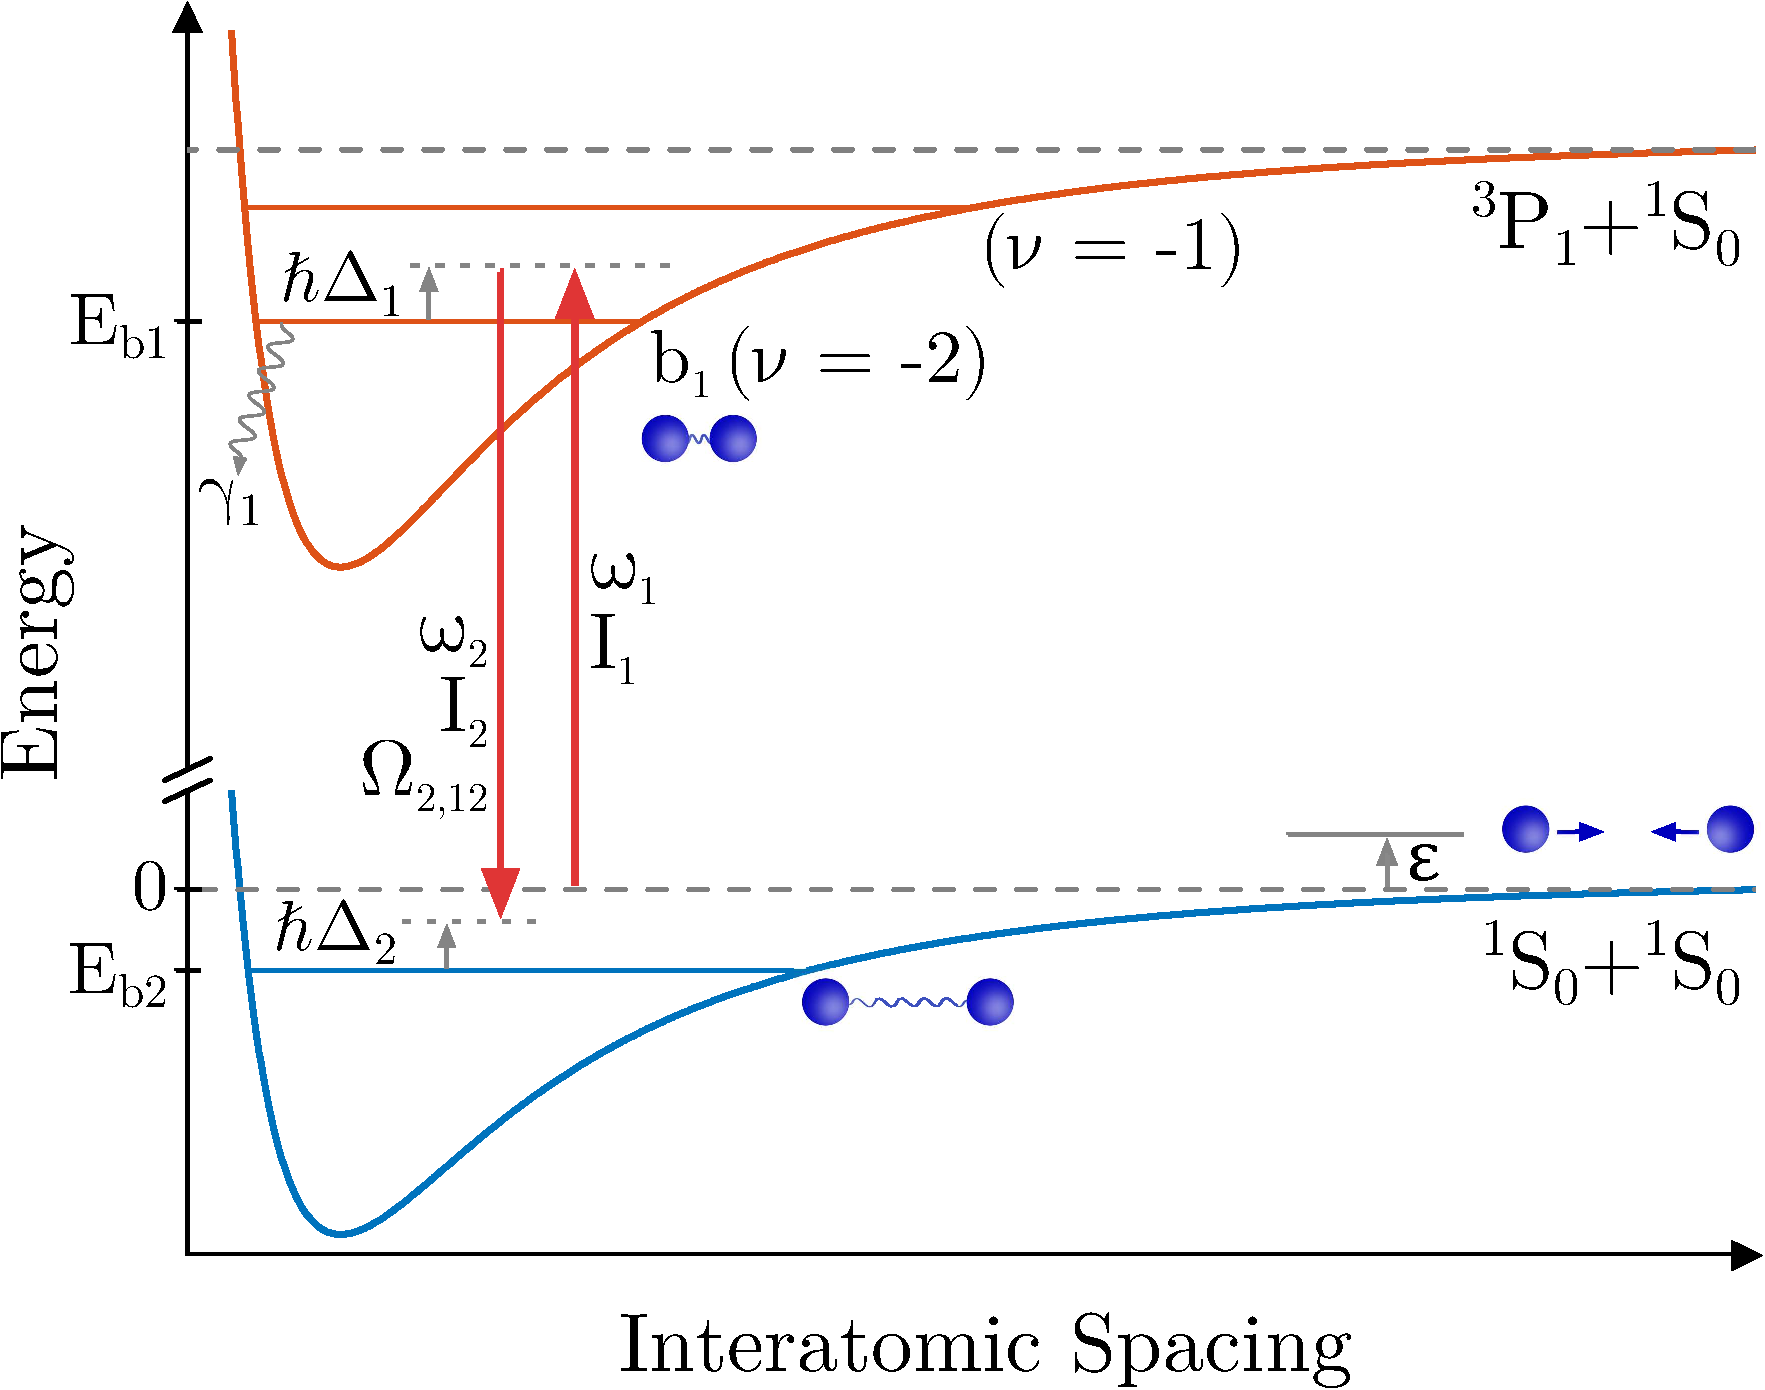
\includegraphics[width=\textwidth]{sr_pa_potential.pdf}}
  \caption{Strontium PAS potential}{Two-photon photoassociation diagram . The energy of two well-separated $^1S_0$ atoms at rest is taken as zero. $\epsilon$ is the kinetic energy of the colliding atom pair. $E_{b1}$ is the unperturbed energy of the bound state of the excited molecular potential that is near resonance with the free-bound laser, which in these experiments is the second-least bound level of the excited molecular potential ($\nu=-2$). $E_{b2}$ ($<0$) is the unperturbed energy of the least bound state of the ground molecular potential. The photon of energy $\hbar \omega_1$ is detuned from $E_{b1}$ by $\hbar \Delta_1$ for $\epsilon=0$, while the two-photon detuning from $E_{b2}$ is $\hbar \Delta_2$. The decay rate of $b_1$ is $\gamma_1$. Stark and collisional frequency shifts are neglected in this schematic.}
  
%All frequencies are measured with respect to the atomic $^1S_0$-$^1P_1$ transition.
\end{figure}

In this work, we probe the halo state in $^{86}$Sr using two-photon Raman photoassociation (PA) \cite{jtl06}, in which two laser fields couple colliding atoms to the least-bound state of the ground molecular potential. We tune near resonance with an intermediate state that is bound in the $0_u$ potential  corresponding to the $^1S_0+ {^3P_1}$ asymptote at long range \cite{mmp08} (Fig.\ \ref{PASDiagram}). We accurately determine the $^{86}$Sr$_2$ binding energy, considering possible collisional frequency shifts and AC Stark shifts due to trapping and excitation lasers. Using the universal prediction for the binding energy, including corrections derived for a van der Waals potential \cite{gfl93,gao01,gao04}, we derive a more accurate value of the $s$-wave scattering length for $^{86}$Sr atomic collisions \cite{skt10,mmp08}.

%The spin-forbidden $^1S_0$-$
%{^3P_1}$ intercombination transition at $\lambda=689$\,nm is weakly
%allowed due to spin-orbit coupling of the ${^3P_1}$ state with the
%lowest-lying ${^1P_1}$ level \cite{scg04theory}.

% and calculate the scattering length using theory for a weakly bound molecule on a van der Waals potential \cite{gfl93,gao04}.

%A model only accounting for a single excited-state channel \cite{bju96} cannot explain the observed frequency dependence of the AC Stark shift of the two-photon transition. This can be attributed to the proximity of other excited states.

\section{Experimental setup}
\label{sec:lowE_setup}

Regarding the general process 

Using the \intPot{\gs}{\ex} interatomic potential, we perform a raman process using the $\nu=-2$ bound state which has a binding energy of E$_b=-44 \text{MHz}$ \hl{cite improved binding en}. Sample pre 

We used strontium 86 in a thermal gas at temperatures between 30 and 1000 nK. Typical peak densitieis were around $\peakDens{1}{12}$. 

Raman process using the second bound state of the \intPot{\gs}{\ex} interatomic potential

What atom do we use
what is the sample conditions
what trap do we use
what are the dimensions of the trap
what are the trap freq
how do we determine 

%% paper
Two-photon spectroscopy is performed on ultracold $^{86}$Sr atoms in a single-beam optical dipole trap (ODT) generated from a 1064-nm laser propagating perpendicular to gravity with beam waists of $260$\,$\mu$m and $26$\,$\mu$m \cite{mmp08,ssk14}. The tight waist provides vertical confinement. The trap depth after an evaporative cooling stage determines the sample temperature, which is set between $30-1000$\,nK. Typical atom numbers are several hundred thousand and peak densities are as high as $2\times 10^{12}$\, cm$^{-3}$. The number of atoms and sample temperature are measured using time-of-flight absorption imaging operating on the $^1S_0$-$^1P_1$ transition. Trap oscillation frequencies are determined by measuring dipole and breathing collective mode frequencies, which allow determination of trap volume and sample density.

%The lifetime of atoms in the ODT due to collisions with
%background atoms is about $xx\,\textrm{s}$.

%Trap oscillation frequencies measured by the parametric resonance
%technique [PRA 57, R20 (1998)] agree with values calculated from the
%ODT laser power and measured beam waist,
%giving us confidence that we know the geometry of our trap.%confirm our ODT characterization. For a
%single-beam power of 6 W, we measure $\nu_{trap}=215$ Hz in the
%gravitational axis and 155 Hz in the perpendicular axes.


\begin{figure} \label{Experimental Setup}
\centerline{
  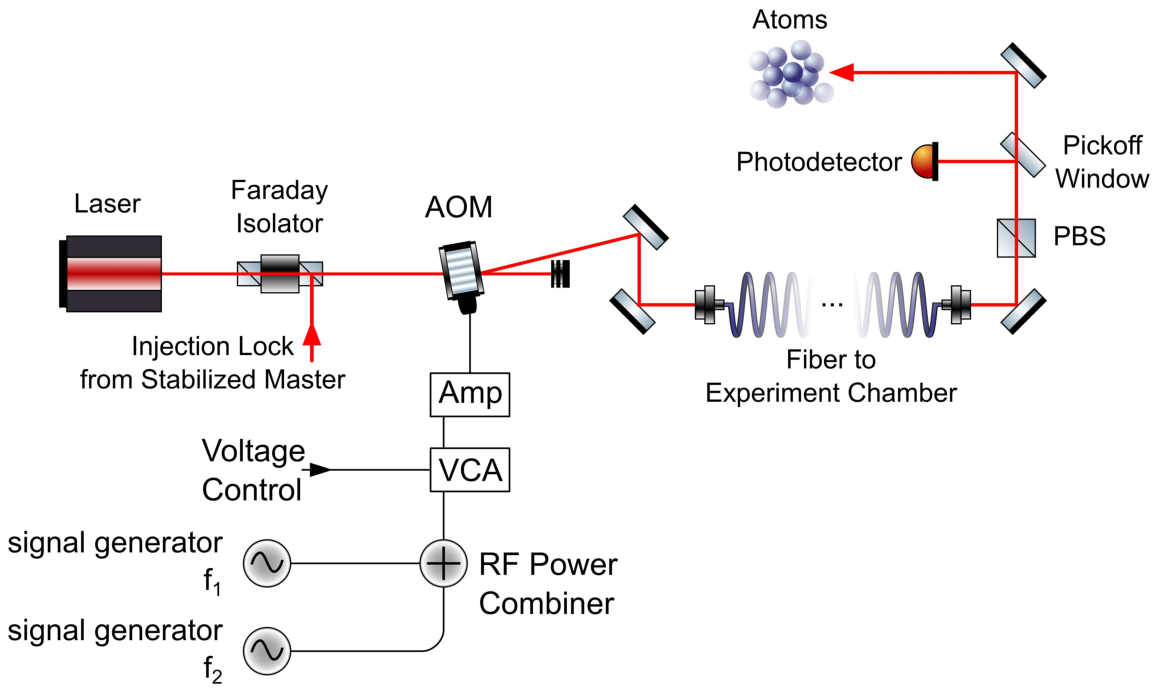
\includegraphics[width=\textwidth]{pa_exp_setup.pdf}}
  \caption{PAS laser setup}{Photoassociation laser schematic . A master laser is frequency-stabilized via saturated absorption spectroscopy to the $^1S_0$-$^3P_1$ atomic transition. After amplification with a diode slave laser, light at two controllable frequencies is generated with a single acousto-optic modulator (AOM) and delivered to the atoms with an optical fiber. The beat note between the two frequencies is monitored after the fiber.}  
\end{figure}


\subsection{Photoassociation}

After the atoms have equilibrated in the final ODT configuration, the PA lasers are applied (Fig.\ \ref{PASDiagram}). A single acousto-optic modulator, driven with two RF frequencies, is used to generate both PA beams. Light is derived from a frequency-stablized master laser (Fig.\ \ref{Experimental Setup}) and coupled into a single-mode optical fiber with output optics that yield a 320\,$\mu$m waist at the atoms, much larger than the size of the atom cloud. Both PA beams are linearly polarized along the same direction. The beat signal of the two light fields after the fiber is monitored on a photodiode and the RF powers are adjusted to ensure matched intensities for the two frequency components ($I_1=I_2\equiv I$).

%$I_{689}$ is varied to obtain the intensity-dependence of the two-photon transition.

%(One could in principle vary the power of both light fields independently and measure how the two-photon line position changes. This will allow us to decouple the contributing factors to the AC Stark shift. If we are going to develop a theory of the multiphoton line, it will have to be able to treat this regime as well. )

The sample temperature is low enough that collisions are entirely $s$-wave. The target state for the two-photon transition has total angular momentum $J=0$ and binding energy $E_{b2}(<0)$. $^{86}$Sr has no nuclear spin and a $^1S_0$ electronic ground state, leading to a single ground electronic molecular potential (X$^1\Sigma_g^+$). The dominant intermediate state ($b_1$) is the $J=1$ rotational state of the second least-bound ($\nu=-2$) vibrational level on the $0^+_u$ molecular potential, which asymptotically connects to the $^1S_0$-$^3P_1$ atomic transition at long range. This state is bound by $44.246(10)$\,MHz \cite{bmc14}. We define $\Delta_1=\omega_1-E_{b1}/\hbar$ and $\Delta_2=\omega_1-\omega_2-E_{b2}/\hbar$ as the one-photon detuning from state $b_1$ and two-photon detuning from state $b_2$ respectively for an initial scattering state with collision energy $\epsilon=0$.
$\Omega_{2,12}$ is the Rabi frequency for coupling between states $b_1$ and $b_2$ due to the laser field at $\omega_2$ with single-beam intensity $I_2$.
Because the binding energy of the halo molecule is very small compared to $\Delta_1$, both laser frequencies are near resonance with the $\nu=-2$ state.  The transitions to the least-bound ($\nu=-1$) $J=1$ excited molecular state, bound by $1.633(1)$\,MHz, and the excited atomic state lie near enough in energy that they can effect our observations.


%Because the binding energy of the halo molecule is very small ($E_{b2}\ll \hbar \Delta_1$), both lasers
%are
%near
%resonance with a single-photon, free-bound transition to$-44.246(10)$\,MHz to the red of
%the $^1S_0$-$^3P_1$ atomic transition \cite{bmc14}. The upper state of this transition is the $J=1$ rotational state of the second least-bound
%vibrational level on the $0^+_u$ molecular potential. The least-bound $J=1$ excited molecular state, bound by $1.633(1)$\,MHz, and the atomic transition lie near enough in energy that they play important roles in our observations.

%Laser $f_1$ is near resonant with a single-photon, free-bound
%transition 222.2\,MHz the red of the $^1S_0$-$^3P_1$ atomic
%transition. This is $J=1$ rotational state of the third least-bound
%vibrational level on the $0u$ molecular potential \cite{zbl06}.

Photoassociation leads to loss of atoms from the trap through radiative decay from the intermediate, excited electronic state, and from collisions between molecules and background atoms. The PA spectrum is obtained by holding $\omega_2$ fixed and varying $\omega_1$, which varies $\Delta_2$ across resonance (Fig.\ \ref{PASDiagram}). $\Delta_1$ thus also varies slightly during a scan, but the spectra are so narrow compared to $\Delta_1$ that we neglect this in our analysis. After an exposure time on the order of one hundred milliseconds, the number of ground-state atoms remaining and the sample temperature are measured with time-of-flight absorption imaging.

%The observed PA spectrum is relatively simple because the
%bosonic isotopes of strontium lack hyperfine structure. As shown in
%Fig.\ \ref{PASDiagram}, ground state $^1S_0$ atoms collide on a
%single $^1\Sigma^+_g$ potential. Four molecular potentials converge
%to the $^1S_0$ + $^3P_1$ asymptote \cite{mjs01}, but only states of
%the $0^+_u$ and $1_u$ potentials are optically connected to the
%$^1\Sigma^+_g$ potential \cite{zbl06}. At the low temperatures of
%these experiments, only $s$-wave collisions occur so only $J=1$
%intermediate levels and $J=0$ and 2 final states can be populated.



%\section{Details of the Model of the Photoassociation Lineshape}
%\label{sectionappendix}



%The effective volumes used throughout this analysis are defined by
%\begin{equation}\label{eq:effectivevolumes}
%	V_{\text{q}}=\int_{\mathrm{V}} d^3r \, e^{-\frac{qU(\mathbf{r})}{k_{B}T}},
%\end{equation}
%for trapping potential $U(\mathbf{r})$.

%The collision event rate constant can be expressed as a thermal average of the scattering probability for loss, $\vert S(\epsilon,\omega_1,\omega_2,...,\mathbf{r})\vert^2$, over the collision energy $\epsilon$. 

%We also average over the trap volume to allow for the possibility that the scattering probability can vary with position in the trap due to inhomogeneity of laser intensity profiles and the density distribution [Eq.~(\ref{equationKeffective})].



%Bohn and Julienne \cite{bju96} provide an expression for $\vert S(\epsilon,\omega_1,\omega_2,...)\vert^2$ for a collision on the open channel of two ground state atoms (g) with total energy $\epsilon$ leading to loss-producing decay from the excited state $b_1$ with rate $\gamma_1$. (See Fig.\ \ref{PASDiagram}.) It yields
%\begin{eqnarray}\label{equationSprob}
%  \vert S\vert^2 =   \hspace{2.5in}&&\\
%  {(\Delta_2+\epsilon/\hbar)^2{\gamma}_1{\gamma}_s \over
%  	\left[(\Delta_1+\epsilon/\hbar)(\Delta_2+\epsilon/\hbar)-\frac{\Omega_{12}^{2}}{4}\right]^2+\left[ \frac{\gamma_1+\gamma_s}{2}\right]^2(\Delta_2+		 	\epsilon/\hbar)^2}, &&\nonumber
%\end{eqnarray}
%where all quantities are defined in the main text. For simplicity, we have omitted the light shift of $b_1$ due to coupling to the scattering continuum \cite{bju99}. Equation (\ref{equationSprob}) neglects all light shifts due to the trapping laser. Light shifts due to the photoassociation lasers coupling to states outside our model (Fig.\ \ref{PASDiagram}) are also neglected. The thermal energy is much greater than the zero-point energy for trap motion, $T\gg h\nu_{\text{trap}}/k_B$, so confinement effects are negligible \cite{zbl06}.




%For the experiments reported here, we maintain significant intermediate-state detuning, $|\Delta_1|\gg |\Omega_{12}|$. Thus we are in a Raman configuration, and near two-photon resonance the expression for the scattering probability for a given initial scattering energy Eq.~(\ref{equationSprob}) can be approximated as a Lorentzian
%\begin{eqnarray}\label{equationSprobLorentzian}
% \vert S\vert^2 \approx {A(\epsilon) \over
% \left(\Delta_2+\epsilon/\hbar-\frac{\Omega_{12}^{2}}{4(\Delta_1+\epsilon/\hbar)}\right)^2+\left[ {\Gamma_L(\epsilon)}/{2}\right]^2},
%\end{eqnarray}
%where $A$ and $\Gamma_L$ are defined in Eqs.\ (\ref{ApproxLorentzianQuantitiesMain}) and (\ref{ApproxLorentzianQuantities-2Main}).
%
%As discussed in the text, we analyze loss spectra using the effective expression, Eq.\ (\ref{equationApproxLorentzian}) to account for possible deviations from the single-channel theory \cite{bju96}.

\subsection{Consideration of the trap depth}
\label{sec:trunc_trap}

Show plots of the trap and how we determined what the trap depth was

Our previous discussion of the rate loss constant assumed we could describe the spatial distribution of the atomic density profile analytically. This is a valid supposition given two key assumptions, 1) the sample termperature remains constant during the PA exposure and 2) the trap is of sufficient depth that we can reasonably approximate it as a harmonic trap. \hl{cite Mi's trap paper}.

Analysis of the trapping conditions after acquisition of the data revealed that this second assumption was not maintained during our experiment. In some figure we can see that we only have an eta of 2. This is troublesome as it means we must numerically consider the density distribution over space when solvinf for the rate loss constant K. 

In addition to the modified spatial distribution, we must also consider the effect of the trap depth on the energy profile of the trapped gas. In a typical high-eta trap, a typical Boltzmann profile is sufficient to describe the velocity distribution of the atoms and when we consider the distribution of relative energies that is important for PAS expeirments, we recover a simple bolztmann weighting for the distribution of energy probabilities. This is shown in \hl{sopme app}.

However, the case of a low-eta trap we must define a local cutoff energy at each point in space within the trap as atoms that have an energy higher than the local eta value are assumed to be lost from the trap. Derivation of this truncated relative energy probabillity distribution is given in \hl{some app} and results in a stronger weighting of the coldest atoms near the bottom of the trap.



\section{Theoretical description}
\label{sec:lowE_theory}

This section develops the more groddy form of the BJ equation. Include the 

In Ch. \hl{somewhere} we discussed the usual situation for observing loss due to photoassocition. This experiment was similar to the 88 autler townes experiment. 

%% paper
PA loss is described with a local equation for the evolution of the atomic density
\begin{equation}\label{densitydecay}
	\dot{n}=-2 Kn^2-\Gamma n,
\end{equation}
where the laser-frequency dependence of the collision-event rate constant, $K$, determines the spectrum of the PA loss. The one-body loss rate, $\Gamma$, is due to background collisions and off-resonant scattering from the PA lasers. By integrating this equation over the trap volume, we can obtain the evolution of the total number of trapped atoms
\begin{equation}\label{number}
   N(t)={N_0 \rm{e}^{-\Gamma t} \over 1+
   {2 N_0 \langle K \rangle V_2\over \Gamma V_1^2}(1-\rm{e}^{-\Gamma t})}
\end{equation}
where $N_0$ is the number of trapped atoms at the beginning of the PAS interaction time. The effective trap volumes $V_q$ are 
\begin{equation}\label{eq:effectivevolumes}
	V_{\text{q}}=\int_{\mathrm{V}} d^3r \, e^{-\frac{qU(\mathbf{r})}{k_{B}T}},
\end{equation}
for trapping potential $U(\mathbf{r})$. 
 $\langle K \rangle$ is the trap-averaged collision event rate constant
\begin{eqnarray}\label{equationKeffective}
  \langle K \rangle&=& \frac{1}{V_{2}}\int_{\mathrm{V}} d^3r \,e^{-\frac{2U(\mathbf{r})}{k_{B}T}} \nonumber \\
  &&\times \frac{1}{h\,Q_{T}} \int_{0}^{\epsilon_{\text{max}}({\mathbf{r}})}d\epsilon \vert S\vert^2 \,e^{-\epsilon/k_{B}T},
\end{eqnarray}
which is itself a thermal average of the scattering probability for loss ($\vert S(\epsilon,\omega_1,\omega_2,...,\mathbf{r})\vert^2$) over the collision energy $\epsilon$, with an energy cutoff $\epsilon_{\text{max}}$ to be discussed momentarily. The trapping potential is given by $U(\mathbf{r})=mgz +h\chi_{1064,\text{g}}I_{1064}(\mathbf{r})-\tilde{U}_{\text{min}}$, where $mgz$ is the gravitational potential at height $z$, $I_{1064}(\vec{r})$ is the intensity of the trapping light, and $\chi_{1064,\text{g}}=11$\,Hz/(W/cm$^2$) \cite{YeKatori2008} is proportional to the polarizability of ground state atoms due to $1064$\,nm light. $\tilde{U}_{\text{min}}$ is subtracted to set the potential at the trap minimum to zero. The spatial integral is restricted to regions around the trapping local minimum with $U(\mathbf{r})$ less than the trap depth \cite{ycm11}. Downhill regions on the other side of the saddle point defining the trap depth are excluded. The laser intensity profile is measured independently, and the potential is found to be consistent with measured trap oscillation frequencies. The partition function is $Q_{T}=\left({2\pi k_{B}T \mu \over h^2}\right) ^{3/2}$ for reduced mass $\mu=m/2$ and sample temperature $T$, for atoms of mass $m$.

Equation (\ref{equationKeffective}) provides the correct thermal average when the collision-energy distribution does not need to be truncated $(\epsilon_{\text{max}}\rightarrow \infty)$. For our data, however, the ratio of sample temperature to trap depth is $k_BT/U_{\text{depth}}\approx 3$ for samples with temperature above $100$\,nK and drops to unity for 30\,nK samples, so truncation effects are important. If the single-particle kinetic-energy distribution function is a Boltzmann truncated at $U_{\text{depth}}-U(\mathbf{r})$, then the collision-energy distribution follows a Boltzmann distribution at low energies $[\epsilon\ll U_{\text{depth}}-U(\mathbf{r})]$ and falls off more quickly at larger energies, reaching zero at $2[U_{\text{depth}}-U(\mathbf{r})]$. We find that this treatment predicts a narrower distribution on the red side of the spectral line than we observe in our data, suggesting the presence of atoms in non-ergodic orbits with energies above the saddle point of the trap. This is not surprising given the large collisional loss rate associated with near-resonant scattering in this isotope. Fortunately, the molecular binding energy is strongly determined by the sharp edge of the spectrum on the blue side of the line, which is relatively insensitive to the description of the red tail. Our data is fit well with a truncated Boltzmann distribution of collision energies [Eq.~(\ref{equationKeffective})]. To estimate the systematic uncertainty introduced by this treatment, we perform fits with $\epsilon_{\text{max}}$ equal to $2[U_{\text{depth}}-U(\mathbf{r})]$ and $U_{\text{depth}}-U(\mathbf{r})$ and take the mean of the two results as the best value for the binding energy and half the difference as a systematic uncertainty $\sigma_{\epsilon_{\text{max}}}\approx 100$\,Hz. This procedure does not correctly represent the overall normalization of $\langle K \rangle$, but we are not concerned with overall signal amplitude in this study. Atom temperatures vary by no more than 20\% during the interaction time, so assuming a constant sample temperature is reasonable.

%\textit{Unless otherwise stated, we ensure that the change in sample temperature is small during the laser excitation so that assumptions of thermal equilibrium and constant temperature are reasonable.}

%bound by 222.161\,MHz \cite{zbl06} is utilized in this work.

%Bohn and Julienne \cite{bju96} provide an expression for $\vert S(\epsilon,\omega_1,\omega_2,...)\vert^2$ for a collision on the open channel of two ground-state atoms (g) with total energy $\epsilon$ leading to loss-producing decay from the excited state $b_1$ with rate $\gamma_1$. (See Fig.\ \ref{PASDiagram}.
%More details are provided in App.\ \ref{sectionappendix}). This approach was found to be sufficient for describing two-photon spectroscopy to a more deeply bound molecular level in $^{88}$Sr \cite{mmp08}.

Bohn and Julienne \cite{bju96} provide an expression for $\vert S(\epsilon,\omega_1,\omega_2,...)\vert^2$ for a collision on the open channel of two ground state atoms (g) with total energy $\epsilon$ leading to loss-producing decay from the excited state $b_1$ with rate $\gamma_1$ (Fig.\ \ref{PASDiagram}),
\begin{eqnarray}\label{equationSprob}
  \vert S\vert^2 =   \hspace{2.5in}&&\\
  {(\Delta_2+\epsilon/\hbar)^2{\gamma}_1{\gamma}_s \over
  	\left[(\Delta_1+\epsilon/\hbar)(\Delta_2+\epsilon/\hbar)-\frac{\Omega_{12}^{2}}{4}\right]^2+\left[ \frac{\gamma_1+\gamma_s}{2}\right]^2(\Delta_2+		 	\epsilon/\hbar)^2}. &&\nonumber
\end{eqnarray}
 For simplicity, we have omitted the light shift of $b_1$ due to coupling to the scattering continuum \cite{bju99}.  This approach was found to be sufficient for describing two-photon spectroscopy to a more deeply bound molecular level in $^{88}$Sr \cite{mmp08}. Equation (\ref{equationSprob}) neglects all light shifts due to the trapping laser. Light shifts due to the photoassociation lasers coupling to states outside our model (Fig.\ \ref{PASDiagram}) are also neglected. The thermal energy is much greater than the zero-point energy for trap motion, $T\gg h\nu_{\text{trap}}/k_B$, so confinement effects are negligible \cite{zbl06}.
${\gamma}_{1}=2\gamma_{\text{atomic}}$, where $\gamma_{\text{atomic}}=4.7\times 10^4$\,s$^{-1}$ is the decay rate of the atomic $^3P_1$ level. ${\gamma}_{s}(\epsilon)$ is the stimulated width of $b_1$ due to coupling to the initial scattering state by laser 1, which for low energy can be expressed as \cite{ctj06,bmc14,Pachomow2017a}
\begin{equation}\label{equationstimulatedwidth}
	{\gamma}_{s}(\epsilon)=2k l_{\text{opt}} \gamma_1,
\end{equation}
where the optical length ($l_{\text{opt}}\propto I_1$) is related to the overlap between the initial colliding state and $b_1$, and $k=(2\mu \epsilon)^{1/2}/\hbar$. We take the intermediate state $b_1$ as the $\nu=-2$ state, for which $l_{\text{opt}}/I=(1.5\pm0.3)\times 10^4\,a_0\mathrm{/(W/cm^2)}$ \cite{bmc14}, where $a_0=5.29\times 10^{-11}$\,m is the Bohr radius.

For the experiments reported here, we maintain significant intermediate-state detuning, $\Delta_1$, for which $|\Delta_1|\gg |\Omega_{2,12}|$. Thus we are in a Raman configuration, and not in the Autler-Townes regime \cite{mmp08}.  In the Raman regime, Eq.\ \ref{equationSprob} shows a maximum near two-photon resonance at $\Delta_2+\epsilon/\hbar =\Omega_{2,12}^2/4\Delta_1$. Following a treatment discussed recently for a similar experiment in calcium \cite{Pachomow2017a}, if the detuning is restricted to near two-photon resonance then $\vert S\vert^2$ can be approximated as a Lorentzian
\begin{eqnarray}\label{equationSprobLorentzian}
 \vert S\vert^2 \approx {A(\epsilon) \over
 \left(\Delta_2+\epsilon/\hbar-\frac{\Omega_{12}^{2}}{4(\Delta_1+\epsilon/\hbar)}\right)^2+\left[ {\Gamma_L(\epsilon)}/{2}\right]^2},
\end{eqnarray}
where 
%$A$ and $\Gamma_L$ are defined in Eqs.\ (\ref{ApproxLorentzianQuantitiesMain}) and (\ref{ApproxLorentzianQuantities-2Main}).
\begin{eqnarray}\label{ApproxLorentzianQuantitiesMain}
  A(\epsilon)&=& \frac{\Omega_{2,12}^{4}\gamma_1 \gamma_s(\epsilon)}{16(\Delta_1+\epsilon/\hbar)^4} \\
  \label{ApproxLorentzianQuantities-2Main}
  \Gamma_L(\epsilon)&=& \frac{\Omega_{2,12}^{2}[\gamma_1 +\gamma_s(\epsilon)]}{4(\Delta_1+\epsilon/\hbar)^2}.
\end{eqnarray}
In practice, the variation of collision energy is negligible compared to the one-photon detuning $\Delta_1$. 


%for various detunings from the intermediate state $\Delta_1$ in order to extract parameters such as matrix elements, but
%The smallest detuning is $|\Delta_1|/2\pi=1.5$\,MHz, and

%in which $\hbar\omega_1$ is far off resonance,

%, and we expect to see atom loss when we are approximately on two-photon resonance.
 %We record spectra at fixed $\Delta_1$ by scanning $\Delta_2$.

%$\Delta_2\approx \Omega_{12}^2/4\Delta_1-\epsilon/\hbar$,


There are several concerns regarding the rigorous application of the Bohn and Julienne theory \cite{bju96}  to our experiment. The obvious one is that it assumes an isolated intermediate state, which is not always a good approximation because of the proximity of state $b_1$ to the $^1S_0+{^3P_1}$ asymptote and to the $\nu=-1$ state. Because of the small decay rate $\gamma_1$ of the intermediate molecular state associated with metastable $^3 P_1$ atomic state, we also expect that loss from the ground molecular state cannot be neglected.


The more subtle issue is that Eq.\ (\ref{equationSprobLorentzian}) is derived assuming only a single laser beam is near resonant with each leg of the two-photon transition, which is not a good approximation for two-photon spectroscopy of a halo state and the resulting small laser-frequency difference $\omega_1-\omega_2 \approx -E_{b2}\ll |\Delta_1|$. We can expect that coupling between pairs of states due to both photoassociation lasers will contribute to the transition strength and light shifts of the levels induced by the photassociation lasers \cite{bju96,bju99}.

%The more subtle issue is that Eq.\ \ref{equationSprob} \cite{bju96} assumes that $|E_{b2}|\gg |\Delta_1|\gg |\Delta_2|$ so that to a good approximation laser 1 only couples states $|\varepsilon\rangle$ and $|1\rangle$, and laser 2 only couples states $|1\rangle$ and $|2\rangle$. However, this condition is violated for photoassociation of Halo states, for which $|E_b|$ is very small. In the Raman configuration we use here,
%$|\Delta_1|\gg |E_b|$.


In the absence of a more complete theory treating these effects, we analyze loss spectra using the effective expression given by Eq.\ (\ref{equationApproxLorentzian}), where the observed molecular binding energy ($E'_{b2}$) includes any perturbations due to AC Stark or collisional shifts.
\vbox{
\begin{eqnarray}\label{equationApproxLorentzian}
  \vert S\vert^2 = \frac{\Gamma_L(\epsilon)+\gamma_{\text{eff}}}{\Gamma_L(\epsilon)}\hspace{1.5in} \nonumber \\
  \times \frac{\eta  A(\epsilon)} {\left(\omega_1-\omega_2+\epsilon/\hbar-E'_{b2}/\hbar\right)^2+\left[
  	\frac{\Gamma_L(\epsilon)+\gamma_{\text{eff}}}{2}\right]^2},
\end{eqnarray}}

%-E_{b2}/\hbar-\frac{\Omega_{12}^{2}}{4(\Delta_1+\epsilon/\hbar}
 %$A^T$ and $\Gamma^T_L$ are evaluated at the laser intensities appropriate for the data set being fit and for the collision energy set to a characteristic value for the sample temperature $T$, $\epsilon^T=k_B T$ with Boltzmann constant $k_B$,


Parameters have been added in Eq.\ (\ref{equationApproxLorentzian}) to account for deviations of the signal strength ($\eta$) and width ($\gamma_{\text{eff}}$) from the predictions of   \cite{bju96}. If deviations from Eq.\ (\ref{equationSprobLorentzian}) are small, we expect $\eta\sim1$, $\gamma_{\text{eff}}\sim 0$, and $E'_{b2}\sim E_{b2}+{\Omega_{2,12}^{2}}/{4(\Delta_1+\epsilon/\hbar)}$.

% The detunings used in Eqs. \ref{ApproxLorentzianQuantitiesMain}-\ref{ApproxLorentzianQuantities-2Main} neglect AC Stark shifts and collisional shifts, which are small compared to $\Delta_1$.

Light shifts (AC Stark shifts) due to the trapping lasers and collisions with ground-state atoms (density $n$) should contribute to shifts of molecular resonance. Similar effects were taken into account in a recent, high-precision study of weakly bound molecular states of ultracold ytterbium atoms \cite{bbc17}. In addition, we expect that both 689-nm excitation lasers will shift the line, not just $I_2\propto \Omega_{2,12}^{2}$. We model the relationship between the measured resonance positions and the unperturbed binding energy $E_{b2}$ as
\begin{equation}\label{Eq:GlobalFit}
	E'_{b2}=E_{b2}+h\chi_{689}I_{689}+h\chi_{1064}I_{1064}(\mathbf{r})+h\chi_{n}n(\mathbf{r}).
\end{equation}
The susceptibilities, in Hz per unit intensity or density, will be determined from experimental data or theoretical considerations. The variation with position of the trapping laser intensity ($I_{1064}$) and the density give rise to the spatial dependence of $|S|^2$ and the need for a spatial average in Eq.\ (\ref{equationKeffective}). We take $I_{689}$ as twice the single-beam intensity $I_{689}=2I$. The 689-nm excitation beam is large enough compared to the atom sample to neglect spatial variation. The functional form for the AC Stark shift due to the excitation lasers is discussed in Sec.\ \ref{sectionACStark}.


%, but the correct description of the AC Stark shift due to the excitation laser fields is an open question \textit{(Change this section after getting the conclusion from simulation)} because the intensity of the light field at 689 nm oscillates at frequency $\Delta_2$ with 100\% contrast.

%We take $I_{689}$ as the single-beam intensity $I_{689}=2I$. The correct description of the AC Stark shift due to the excitation laser fields is an open question because the intensity of the light field at 689 nm oscillates at frequency $\Delta_2$ with 100\% contrast, here we neglect this oscillation and assume the AC Stark shift reflects to average total intensity due to the two excitation beams. The 689 nm excitation light is large enough compared to the atom sample to neglect spatial variation.

\begin{figure} \label{Fig:Spectraminus9MHzVaryTrapCold}
\centerline{
  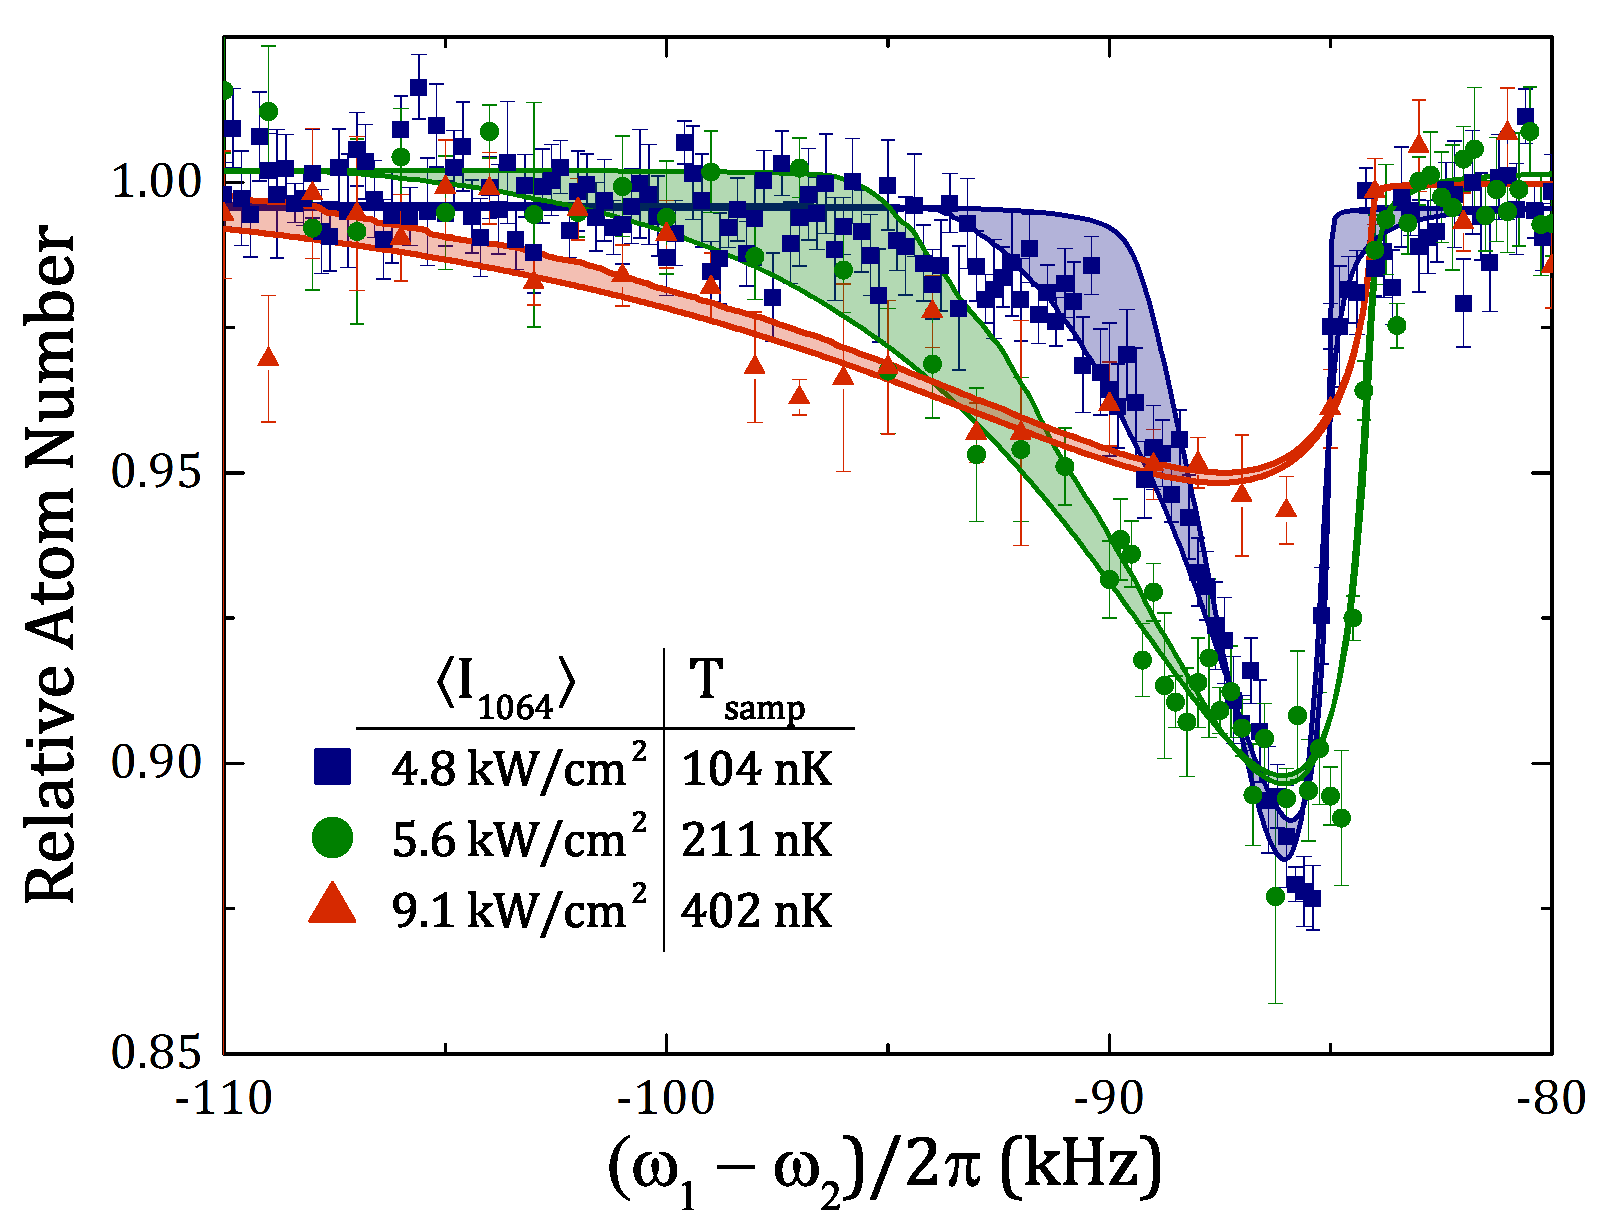
\includegraphics[width=\textwidth]{spectra_vary_1064.pdf}}
  \caption{Variation of 1064 nm trap depth}{Atom-loss spectra as a function of two-photon difference frequency $(\omega_1-\omega_2)/2\pi$ for intermediate detuning
$\Delta_1/2\pi=-9$\,MHz . Sample temperature and average trapping laser intensity are indicated in the legend. The single-beam excitation laser intensity is $I=25$\,mW/cm$^{2}$ for the 104\,nK spectrum and $I=48$\,mW/cm$^{2}$ for the 211\,nK and 402\,nK spectra. Fits are described in the text, with the two boundaries of each band given by the fits with collision-energy truncation
$\epsilon_{\text{max}}$ equal to $2[U_{\text{depth}}-U(\mathbf{r})]$ and $U_{\text{depth}}-U(\mathbf{r})$.}
\end{figure}

\section{Spectral fitting and determination of the binding energy}
\label{sec:lowE_Eb2}

%% paper
%The excitation intensity is $I=0.10$\,mW/cm$^{-2}$ and the intermediate detuning is
%$\Delta_1=-9$\,MHz.
%The peak intensity for the optical dipole trap at the end of the evaporationis indicated in the figure, along with the
%peak initial sample density at the beginning of laser excitation.

Figure \ref{Fig:Spectraminus9MHzVaryTrapCold} shows a series of spectra for different final trap depths and sample temperatures. The characteristic asymmetric lineshape for excitation of a thermal sample is evident, with width decreasing as sample temperature decreases. The molecular binding energy is close to the sharp edge on the blue side of each spectrum.

We fit atom-loss spectra with Eq.\ (\ref{number}) for the evolution of atom number with time, using the phenomenological expression Eq.\ (\ref{equationApproxLorentzian}) for the scattering probability and Eq.\ (\ref{equationKeffective}) for the average of the collision event rate constant over the trap volume and collision energy. The sample temperature, perturbed resonance frequency $E'_{b2}$, $\eta$, and $\gamma_{\text{eff}}$ are taken as fit parameters. In the final analysis, temperatures are set to values determined from time-of-flight imaging of the atoms, but when they are allowed to vary, the fit values differ by no more than 10\%. Approximately 10 spectra are recorded for each set of experimental parameters, and the spread of resulting fit values are used to determine best values and uncertainties.


\subsection{AC Stark Shift due to Excitation Lasers}

\begin{figure} \label{Fig:SpectraVarying689Intensity}
\centerline{
  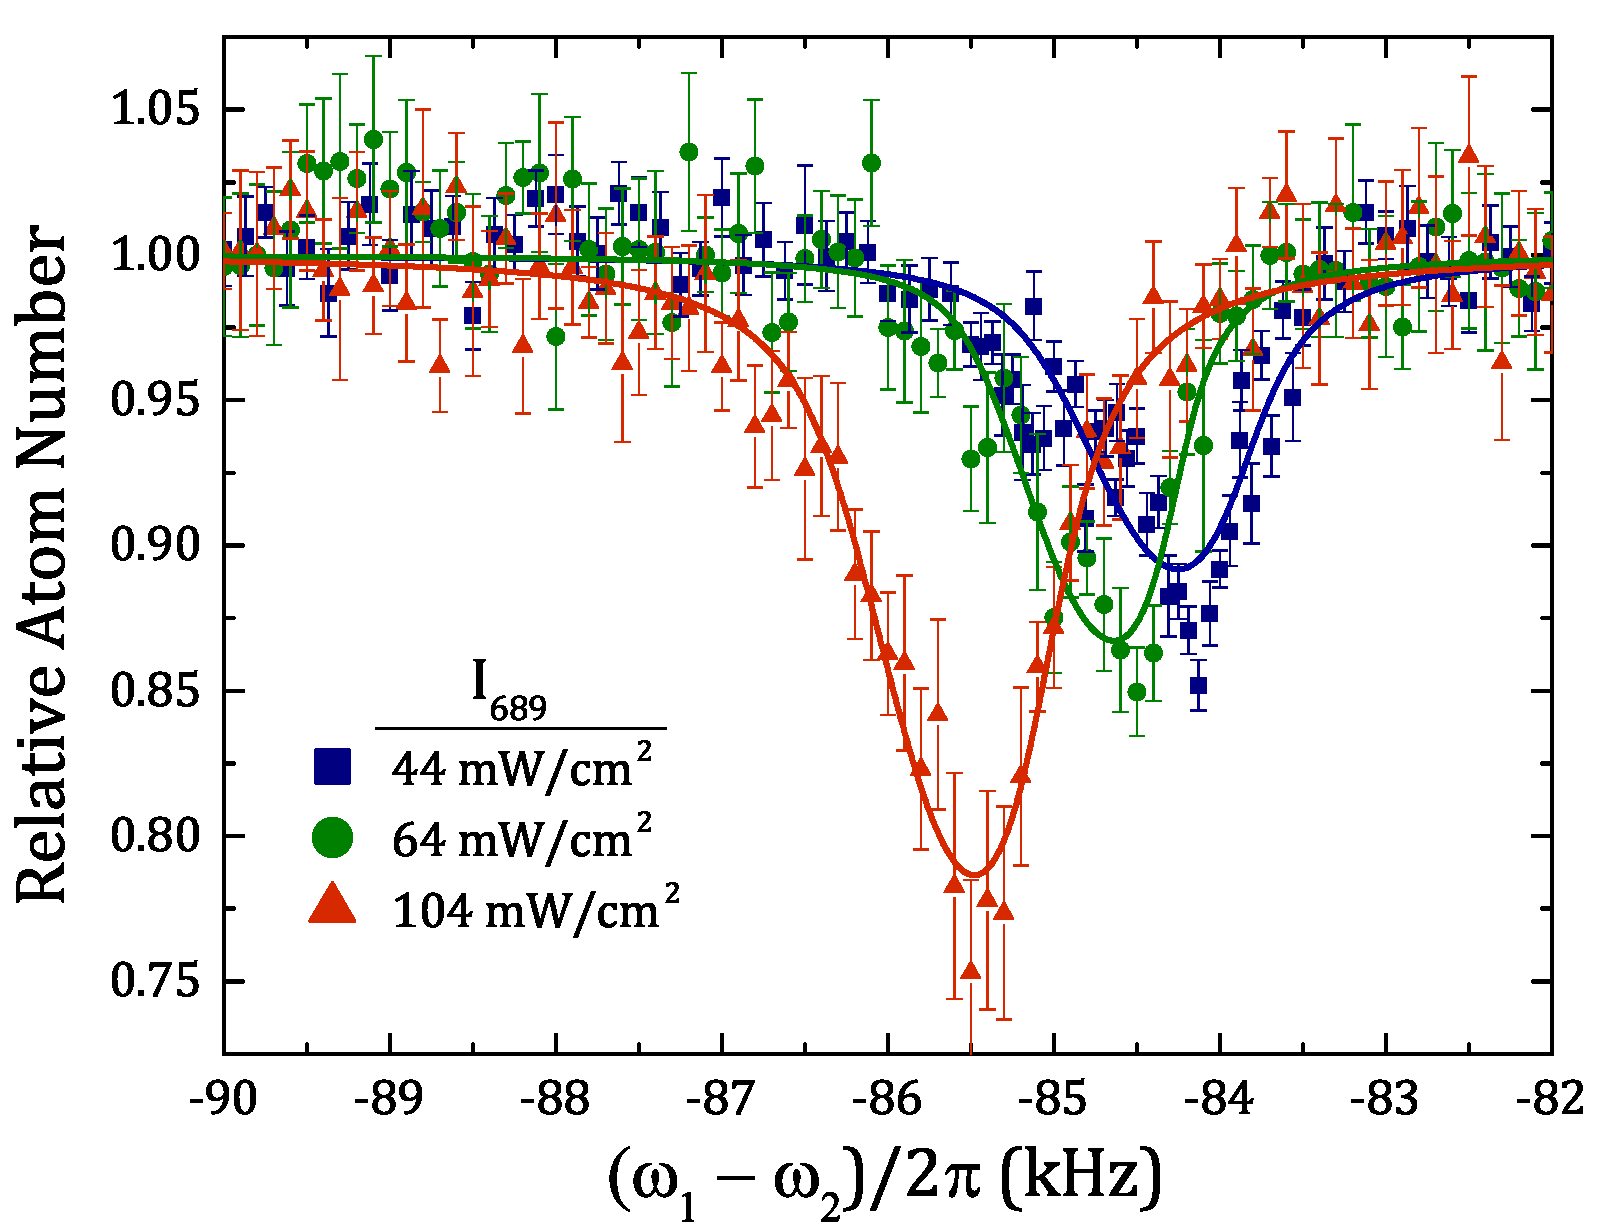
\includegraphics[width=\textwidth]{spectra_vary_689.pdf}}
  \caption{Variation of 689 nm excitation}{Atom-loss spectra as a function of two-photon difference frequency $(\omega_1-\omega_2)/2\pi$ for intermediate detuning $\Delta_1/2\pi=-9$\,MHz and various 689-nm excitation laser intensities . Twice the single-beam intensity $I_{689}=2I$ is indicated in the legend.}
 
\end{figure}

\begin{figure}
\centerline{
  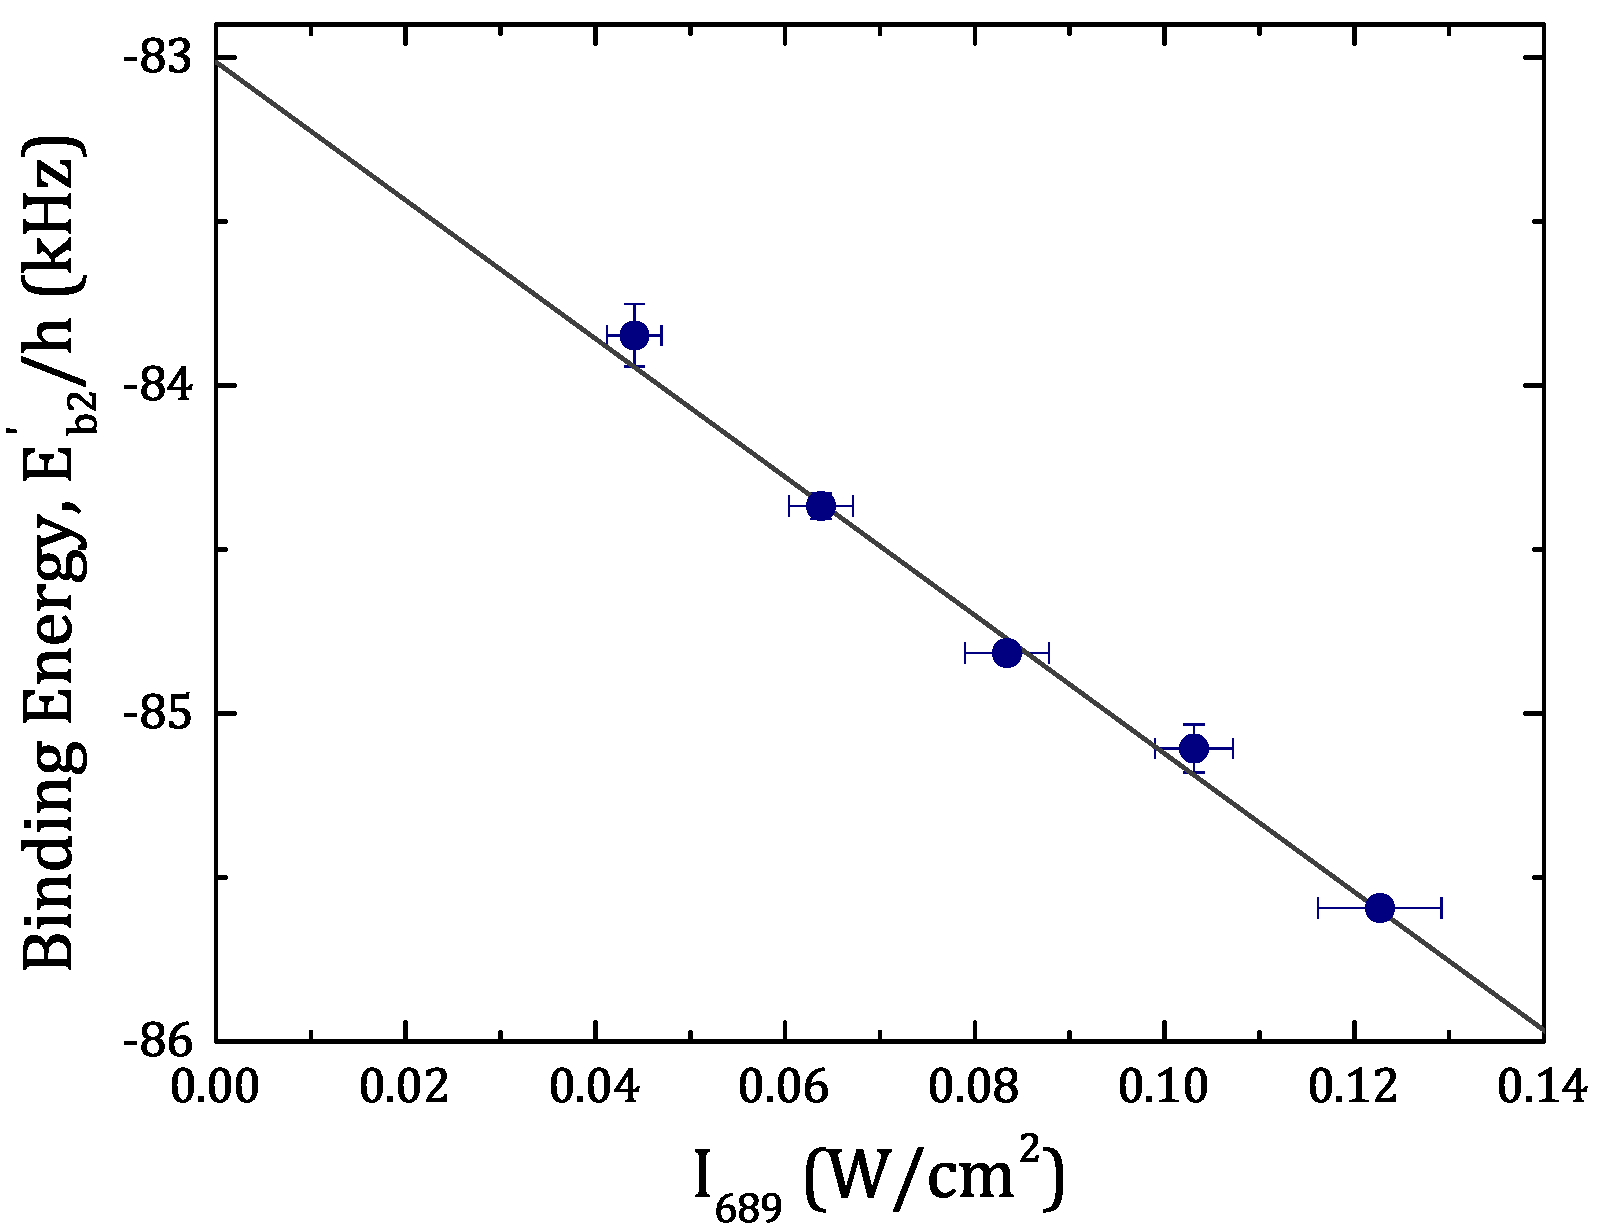
\includegraphics[width=\textwidth]{halo_susceptibility_689.pdf}}
  \caption{Fit of 689 nm AC Stark shift}{Measured resonance position $E_{b2}'$ plotted versus twice the single-beam intensity $I_{689}=2I$ . The linear fit provides the AC Stark shift parameter $\chi_{689}$.}
  \label{Fig:ShiftWith689Intensity}
\end{figure}

The most significant perturbation to the resonance position is the AC Stark shift due to the excitation laser intensity, as shown in Fig.\ \ref{Fig:SpectraVarying689Intensity}. For this data, the trap parameters, temperature ($T=30$\,nK), and initial peak sample density ($n_0=2\times 10^{12}$\,cm$^{-3}$) are held constant. We vary the single-beam excitation intensity from $I=0.02-0.06$\,mW/cm$^{-2}$, and the excitation time is 50\,ms.
The observed shifts are comparable to the thermal width of the spectrum, allowing a precise determination of $\chi_{689}=-21(1)(2)$\,kHz/(W/cm$^{2})$ from a linear fit to the resonance positions, $E'_{b2}\propto h\chi_{689} I_{689}$ (Fig.\ \ref{Fig:ShiftWith689Intensity}). The first quoted uncertainty is statistical and it arises from variations in parameters and fluctuations in the measured intensity during the scans. The second value is systematic, reflecting uncertainty in laser-beam size and intensity profile at the atoms. All parameters beside the 689-nm laser intensity are held fixed for this data set, and the AC Stark shift is not correlated with any other variable, such as density or trap intensity. We thus obtain an accurate measure of $\chi_{689}$ without attempting to account for other systematic shifts of $E'_{b2}$ in this data. A study of the dependence of $\chi_{689}$ on detuning from the excited molecular state
will be discussed in Sec.\ \ref{sectionACStark}.

Broadening to the red of the spectrum reflects the distribution of atom-atom collision energies, while broadening to the blue is most sensitive to decay of the intermediate state ($\Gamma_L$) and the phenomenological broadening term $\gamma_{\text{eff}}$ [Eqs.\ (\ref{ApproxLorentzianQuantities-2Main}) and (\ref{equationApproxLorentzian})]. The long lifetime of the excited state and the significant detuning $\Delta_1$ result in a width $\Gamma_L(\epsilon)$ less than 5\,Hz for all conditions. This is extremely small compared to observed width, which yields values of $\gamma_{\text{eff}}$ on the order of 300\,Hz. We hypothesize that this width reflects decay of molecules in the electronic ground-state due to collisions with background atoms.

\subsection{Density-dependent Frequency Shift}
A shift of the two-photon resonance position is possible due to differing mean-field shifts of initial atomic and final molecular states arising from interaction with the background of ground-state atoms. Such a shift would be proportional to the atom density and depend upon the $s$-wave scattering lengths for atom-atom and atom-dimer collisions, $a_{86}$ and $a_{\text{ad}}$ respectively. This was observed in a Rb Bose-Einstein condensate (BEC) in \cite{wfh00}. For a non-degenerate gas, this effect yields $\chi_n=\hbar (\frac{a_{\text{ad}}}{\mu_{\text{ad}}}-4\frac{a_{86}}{\mu_{\text{aa}}})=\frac{\hbar}{m} (\frac{3 }{2}a_{\text{ad}}-8 a_{86})$, where $\mu_{\text{ad}}$ and $\mu_{\text{aa}}$ are the reduced masses for molecule-atom and atom-atom collisions respectively. Note that the shift would vanish for $a_{\text{ad}}=(16/3) a_{86}$.

The largest density used in our experiment ($\sim 1\times 10^{12}\,\mathrm{cm}^{-3}$) is relatively low compared to typical BEC densities, and at this time we are unable to accurately measure a variation of resonance position with density. However, the atom-atom scattering is close to resonance and thus Efimov physics can provide information on $a_{\text{ad}}$ \cite{bha07,nen17} and an estimate of the systematic error introduced by any residual density-dependent frequency shifts. For a zero-range interaction, the atom-dimer scattering length is related to the atom-atom scattering length through the three-body Efimov parameter $\kappa_*$ according to \cite{bha07}
\begin{equation}\label{Eq:EfimovMoleculAtomScatteringLength}
  a_{\text{ad}}=a_{86}\left\{1.46 + 2.15 \mathrm{cot}[s_0 \mathrm{ln} (14.1\kappa_* a_{86}) ]\right\}
\end{equation}
where $s_0=1.006$ \footnote{The Efimov parameter is related to $E^0_{3b}$ through $\kappa_*=(m|E^0_{3b}|/\hbar^2)^{1/2}$, where $E^0_{3b}$ is the binding energy the lowest Efimov trimer would have in the case of resonant atom-atom interactions.}.

In principle, the atom-dimer scattering length can take any value. However, for a deep atom-atom potential, such as for the ground-state strontium dimer \cite{skt10}, there is a universality of the three-body physics that sets $\kappa_*=0.226(2)/l_{\mathrm{vdW}}$ \cite{wie12}. Here, $l_{\mathrm{vdW}}=\left({2\mu C_6}/{\hbar^2}\right)^{1/4}/2=74.6$\,$a_0$ is the van der Waals length associated with the $C_6$ coefficient of the long-range Sr$_2$ ground-state potential. We use $C_6=3.03(1) \times 10^{-76}$\, J\,m$^6$ found from a fit of potential parameters to spectroscopic data \cite{skt10}, which is consistent with a recent \textit{ab initio} calculation \cite{zbb14}. This yields $\kappa_*=5.72\times 10^7$\,m$^{-1}=(330\,a_0)^{-1}$. Equation (\ref{Eq:EfimovMoleculAtomScatteringLength}) then predicts $a_{\text{ad}}=6.4\, a_{86}$, which leads to a small density-dependent frequency shift parameter of $\chi_n=50\,\mathrm{Hz}/(10^{12}\,\mathrm{cm}^{-3})$. A numerical calculation including a finite-range correction for the atom-atom interaction \cite{mwc17} results in $a_{\text{ad}}=3.5\, a_{86}$ and $\chi_n=-90\,\mathrm{Hz}/(10^{12}\,\mathrm{cm}^{-3})$. Thus, a very small shift is expected for the densities used here. We incorporate $\chi_n=0\pm 90 \,\mathrm{Hz}/(10^{12}\,\mathrm{cm}^{-3})$ as a set parameter in our model of the spectrum, where we set the systematic uncertainty to reflect the spread of theory predictions. This uncertainty will be significant for our determination of the unperturbed halo binding energy.



%Figure \ref{Fig:SpectraDensityVariation} shows  spectra for different sample densities varying from $1-5\times 10^{12}$\,cm$^{-3}$, but the same trapping potential and excitation laser parameters. The samples are prepared by evaporating to a fixed trap depth and holding for 100-700\,ms to allow the atom number and peak density to decay due to three-body recombination, evaporation, and background-gas collisions.
%
%Figure \ref{Fig:ShiftWithDensity} shows the measured resonance frequencies as a function of the  peak density at the start of laser excitation. We observe a susceptibility $\chi_n=xx\pm yy$\,Hz/cm$^{-3}$, consistent with zero. The sample temperature also varies from $250-360$\,nK for this data, so there is some variation in the shift of the resonance from the trap-induced AC Stark shift, and we take that into account in our analysis and determination of the best value for $\chi_n$. (Can we state what that effect is?)
%The density in the experiments presented here is approximately 100 times less than in \cite{wfh00}, which precludes us from placing useful limits on $a_{ma}$ based on our measurements.


\subsection{Unperturbed Halo Binding Energy and AC Stark Shift due to Trapping Lasers}

\begin{figure} \label{Fig:ShiftWithTrapIntensity}
 \centerline{
 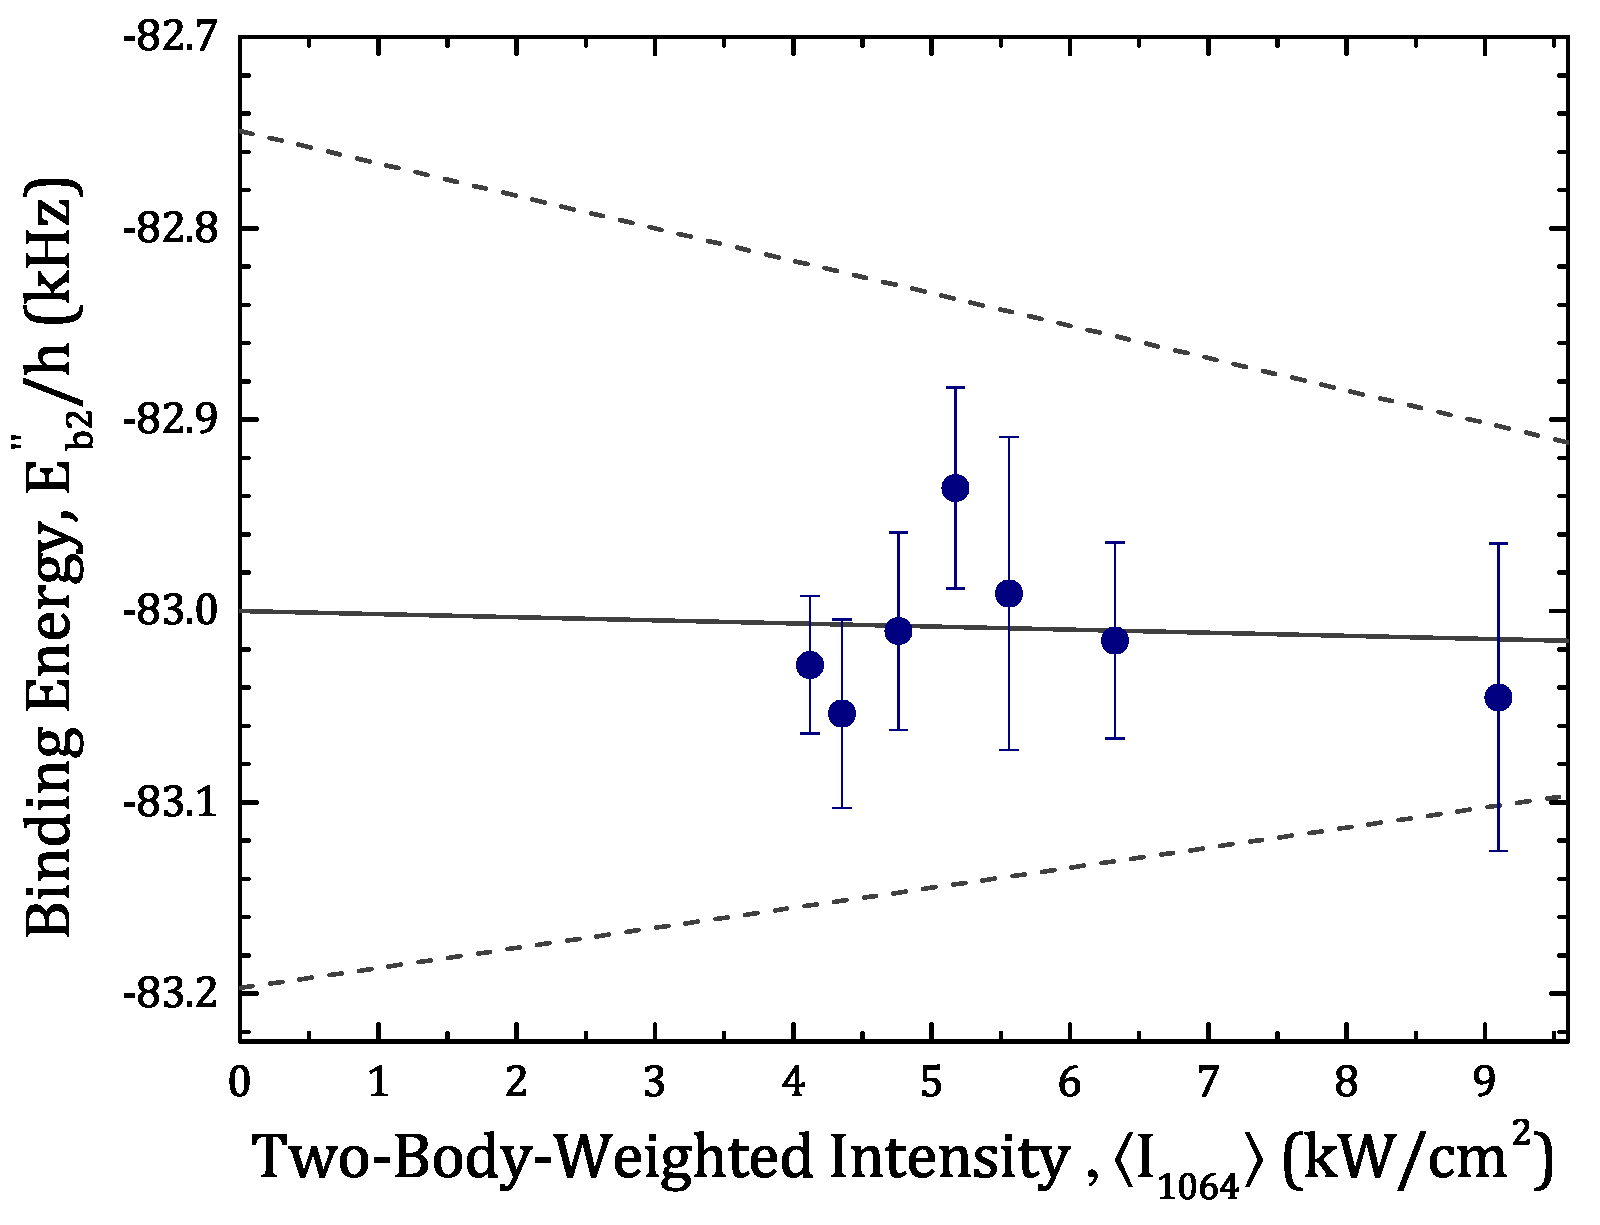
\includegraphics[width=\textwidth]{halo_susceptibility_1064.pdf}}
  \caption{Measurement of halo state susceptibility, $\chi_{1064}$}{Measured resonance positions corrected for excitation-laser AC Stark shift and collisional frequency shift, $E_{b2}'-\chi_{689} I_{689} - \chi_{n}\langle n\rangle$, as a function of average trap laser intensity $\langle I_{1064} \rangle$ for the data such as in Fig. \ref{Fig:Spectraminus9MHzVaryTrapCold} . The trend line and confidence intervals are described in the text.}
\end{figure}

With an accurate determination of $\chi_{689}$ and a value for $\chi_n$, we use the data shown in Fig. \ref{Fig:Spectraminus9MHzVaryTrapCold} to determine the susceptibility for the AC Stark shift from the trapping laser, $\chi_{1064}$, and the unperturbed halo binding energy $E_{b2}$. Figure \ref{Fig:ShiftWithTrapIntensity} shows a plot of $E_{b2}'-\chi_{689}I_{689} - \chi_{\text{n}}\langle n\rangle$ versus $\langle I_{1064} \rangle $, where $E_{b2}'$ is the resonance position from each fit and $\langle ... \rangle $ indicates a weighted average of the quantity over the trapped sample, with a weighting given by the square of atom density. This weighting reflects the contribution to photoassociative loss, a two-body process. The plotted uncertainties in $E_{b2}'-\chi_{689}I_{689} - \chi_{\text{n}}\langle n\rangle$ are from statistical variation in the fit parameters. The typical average density is $\langle n\rangle\approx 1\times 10^{12}$\,cm$^{-3}$. The linear fit function is to $E_{b2}+\chi_{1064}\langle I_{1064} \rangle $. In addition to statistical uncertainty, we have systematic uncertainty from $\chi_{\text{n}}$ and treatment of the truncation of the collision-energy integral [Eq.\ (\ref{equationKeffective})]. The dashed lines shown in Fig. \ref{Fig:ShiftWithTrapIntensity} are resulting fits when the values of $E_{b2}'-\chi_{689}I_{689} - \chi_{\text{n}}\langle n\rangle$ are shifted by the sum of these systematic uncertainties. The resulting value for the unperturbed binding energy is $E_{b2}/h=-83.00(7)(20)$\,kHz, where the first uncertainty is statistical, and the second is systematic. We observe a susceptibility to $I_{1064}$ of $\chi_{1064}=0\pm 10$\,Hz/(kW/cm$^2$).


%For two-photon spectroscopy to a weakly bound dimer, it is typical to neglect any potential AC Stark shift due to far-off-resonant trapping lasers because the atoms contribute to the overall polarizability approximately as free atoms. But the high precision of our measurement allows us to detect a small shift. This corresponds to a relative differential polarizability of ${\chi_{1064}}/{2\chi_{1064,\text{g}}g}}={(\chi_{1064,b2}-2\chi_{1064,\text{g}}g})}/{2\chi_{1064,\text{g}}g}}\approx xx$\%.

\section{Discussion of binding energy}
\label{sec:lowE_alt}

%% paper

%The properties of halo molecules have been well studied \cite{kgj06}.
%One of the most interesting features is their universality, meaning that in the extreme, they can be characterized by a single parameter, the s-wave scattering length. For example,

In the limit of extremely small binding energy, and thus resonant atom-atom interactions, the binding energy of a halo molecule is approximately given by \cite{kgj06}
\begin{equation}\label{Eq:HaloEnergyNoCorrections}
	E_b=-\hbar^2/2\mu a^2.
\end{equation}
For interactions described at long-range by the van-der-Waals form, $V(r)=-C_6/r^6$, as with ultracold atoms, a convenient figure of merit for quantifying how accurate this simple expression should be is given by the ratio of the $s$-wave scattering length to the mean scattering length or interaction range, closely related to the van der Waals length through \cite{gfl93,cju05}
\begin{equation}\label{Eq:InteractionRangevdW}
  \bar{a}= l_{\mathrm{vdW}}\frac{\Gamma\left(\frac{3}{4}\right)}{\sqrt{2}\Gamma\left(\frac{5}{4}\right)}.
\end{equation}

%\begin{equation}\label{Eq:InteractionRangevdW}
%  \bar{a}=2^{-3/2}\frac{\Gamma\left(\frac{3}{4}\right)}{\Gamma\left(\frac{5}{4}\right)}\left(\frac{2\mu C_6}{\hbar^2}\right)^{1/4}.
%\end{equation}
%The universal relation $E_b=-\hbar^2/2\mu a^2$ is valid in general very close to a scattering resonance and over all values of scattering length for a zero-range delta-function pseudopotential \cite{hle57,cgj10}.

%\begin{equation}\label{Eq:HaloEnergyLeadingCorrection}
%-\hbar^2/2\mu(a-\bar{a})^2.
%\end{equation}
% This expression has been shown to be accurate for numerous magnetic Feshbach resonances \cite{cgj10,kgj06}, such as in $^{85}$Rb \cite{kgb03,ckt03}.
%Higher order corrections due to

Slightly away from resonance, corrections to the binding energy for the van der Waals potential were worked out in \cite{gao01,gao04}, yielding
\begin{equation}\label{Eq:BindingEnergyGao}
	E_{b2}=-\frac{\hbar^2}{2\mu(a-\bar{a})^2}\left[1+\frac{g_1\bar{a}}{a-\bar{a}}+\frac{g_2\bar{a}^2}{(a-\bar{a})^2} + ... \right],
\end{equation}
where $g_1=\Gamma(1/4)^4/6\pi^2-2=0.918...$ and $g_2=(5/4)g_1^2-2=-0.947...$. The range of validity of this expression is $a \gtrsim 2 \bar{a}$. The accuracy of the first term in this expansion has been experimentally confirmed for various systems such as $^{85}$Rb \cite{ckt03,kgb03}, $^{40}$K \cite{rtb03,msg05} and $^{6}$Li \cite{bar05}. This derivation of Eq.\ (\ref{Eq:BindingEnergyGao}) assumes that the influence of short-range physics, which can be expressed through a quantum defect, varies negligibly from threshold to the molecular binding energy. We expect this to be an excellent approximation, since, as shown in Ref.~\cite{gao01} the corrections are typically less than about $1\%$ even for GHz binding energies.


%The long-range form of the interaction for s-wave collisions, which determines many aspects of atomic scattering at ultracold temperatures,  can be described with a van der Waals form, $V(r)=-C_6/r^6$. %where $C_6=3.03(1) \times 10^{-76} J m^6$  for Sr \cite{skt10}.
%Details of low energy scattering and near-threshold states for  a van der Waals potential have been well studied, and an important length scale was defined in \cite{gfl93} as the mean scattering length or interaction range \cite{cju05}
%\begin{equation}\label{Eq:InteractionRangevdW}
%  \bar{a}=2^{-3/2}\frac{\Gamma\left(\frac{3}{4}\right)}{\Gamma\left(\frac{5}{4}\right)}\left(\frac{2\mu C_6}{\hbar^2}\right)^{1/4},
%\end{equation}
%where $\mu$ is the reduced mass  and $\hbar$ is the reduced Planck's constant.

%$C_6=3.03(1) \times 10^{-76} J m^6$ \cite{skt10} and

%, where $a_0=5.29\times 10^{-11}$\,m is the Bohr radius.
%This value of $C_6$ is consistent with a recent \textit{ab initio} calculation \cite{zbb14}.

For ground-state $^{86}$Sr atoms, $\bar{a}=71.3$\,$a_0$. The most accurate value available for the s-wave scattering length is $a=798 (12)$\,$a_0$ \cite{skt10}, satisfying the requirement of $a\gg \bar{a}$ for the least-bound state on the ground molecular potential to be a halo molecule. Nonetheless, ${\bar{a}}/({a-\bar{a}})=.10$, and the corrections given by Eq.\ (\ref{Eq:BindingEnergyGao}) are significant. Figure \ref{Fig:HaloBindingEnergy} shows the importance of the correction terms.

\begin{figure} \label{Fig:HaloBindingEnergy}
\centerline{
  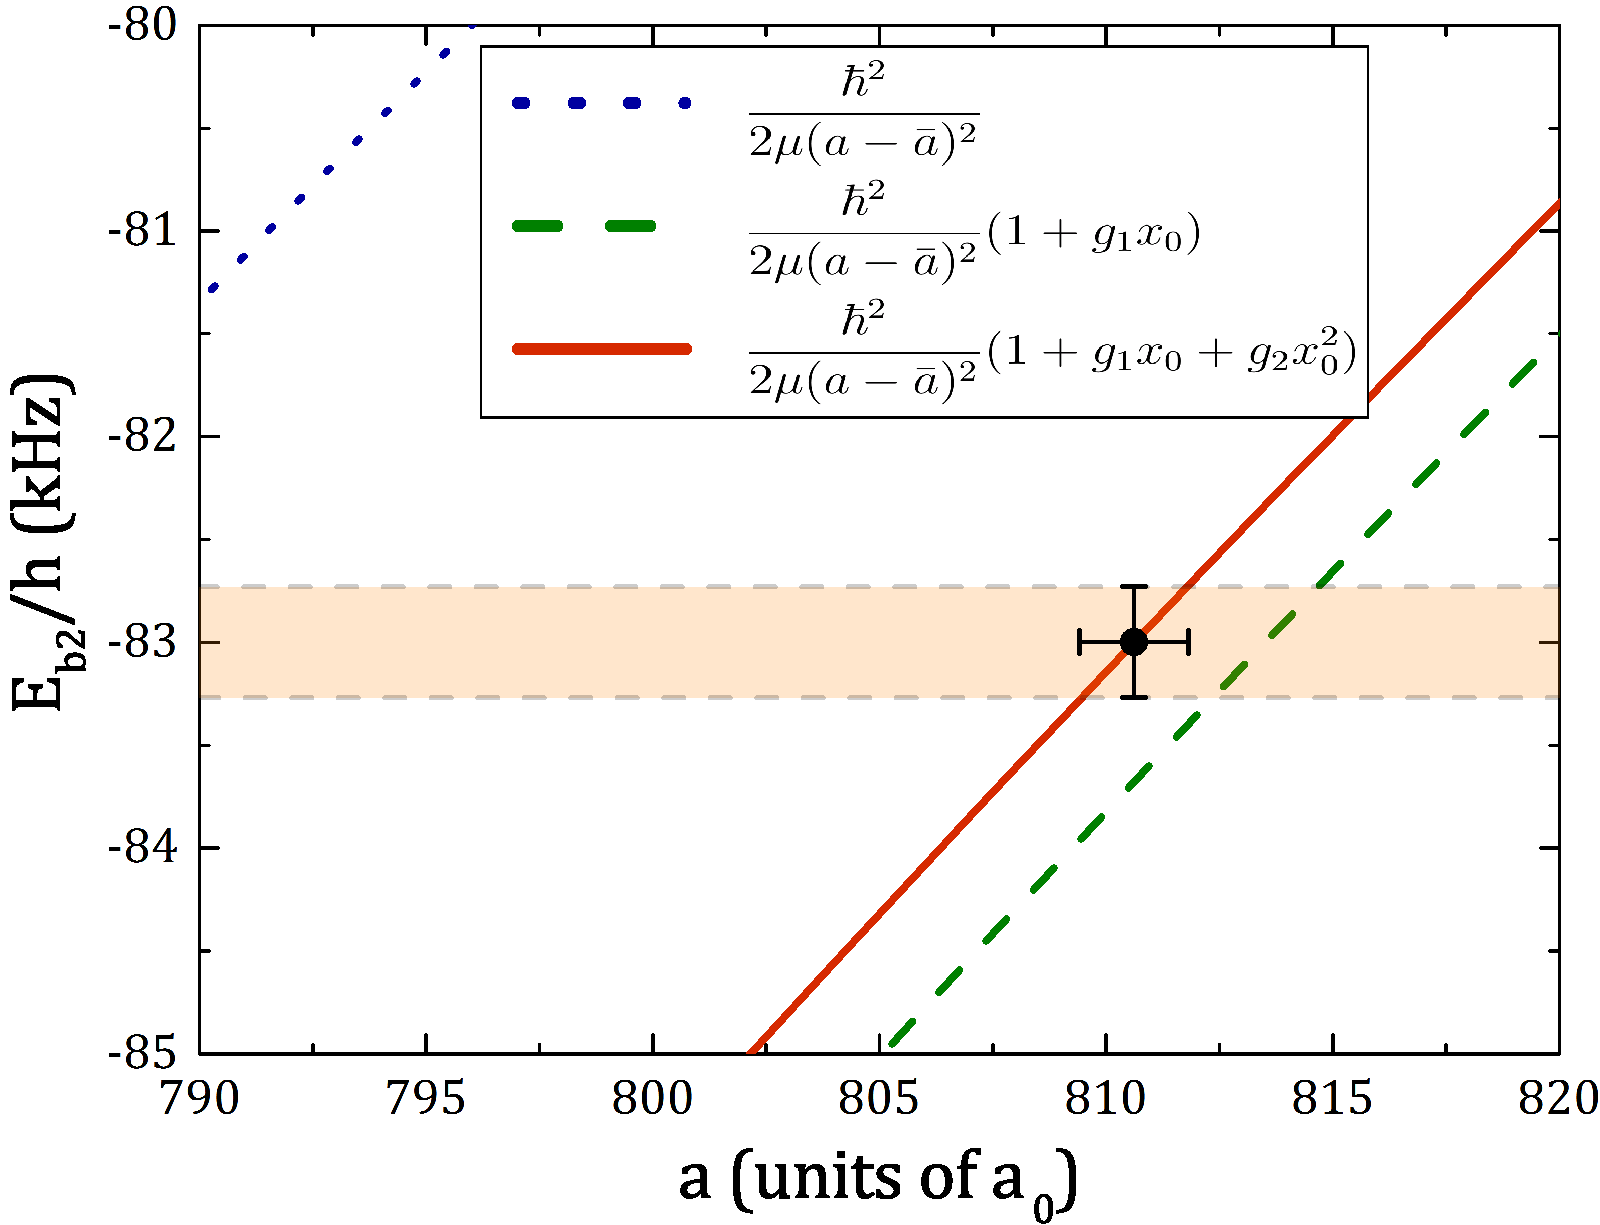
\includegraphics[width=\textwidth]{86_scattering_length.pdf}}
  \caption{Determination of 86 scattering length}{Halo binding energy versus $s$-wave atom-atom scattering length for $^{86}$Sr . The shaded region indicates our experimental measurement. The lines are predictions of Eq.\ \ref{Eq:BindingEnergyGao} retaining up to the first, second, and third terms as indicated in the legend [$x_0={\bar{a}}/({a-\bar{a}})$]. The data point is the prediction of Eq.\ (\ref{Eq:BindingEnergyGao}) for the recommended value of the measured binding energy.}
  
\end{figure}

\begin{figure} \label{Fig:ShiftsofLinesWithIntensity}
\centerline{
  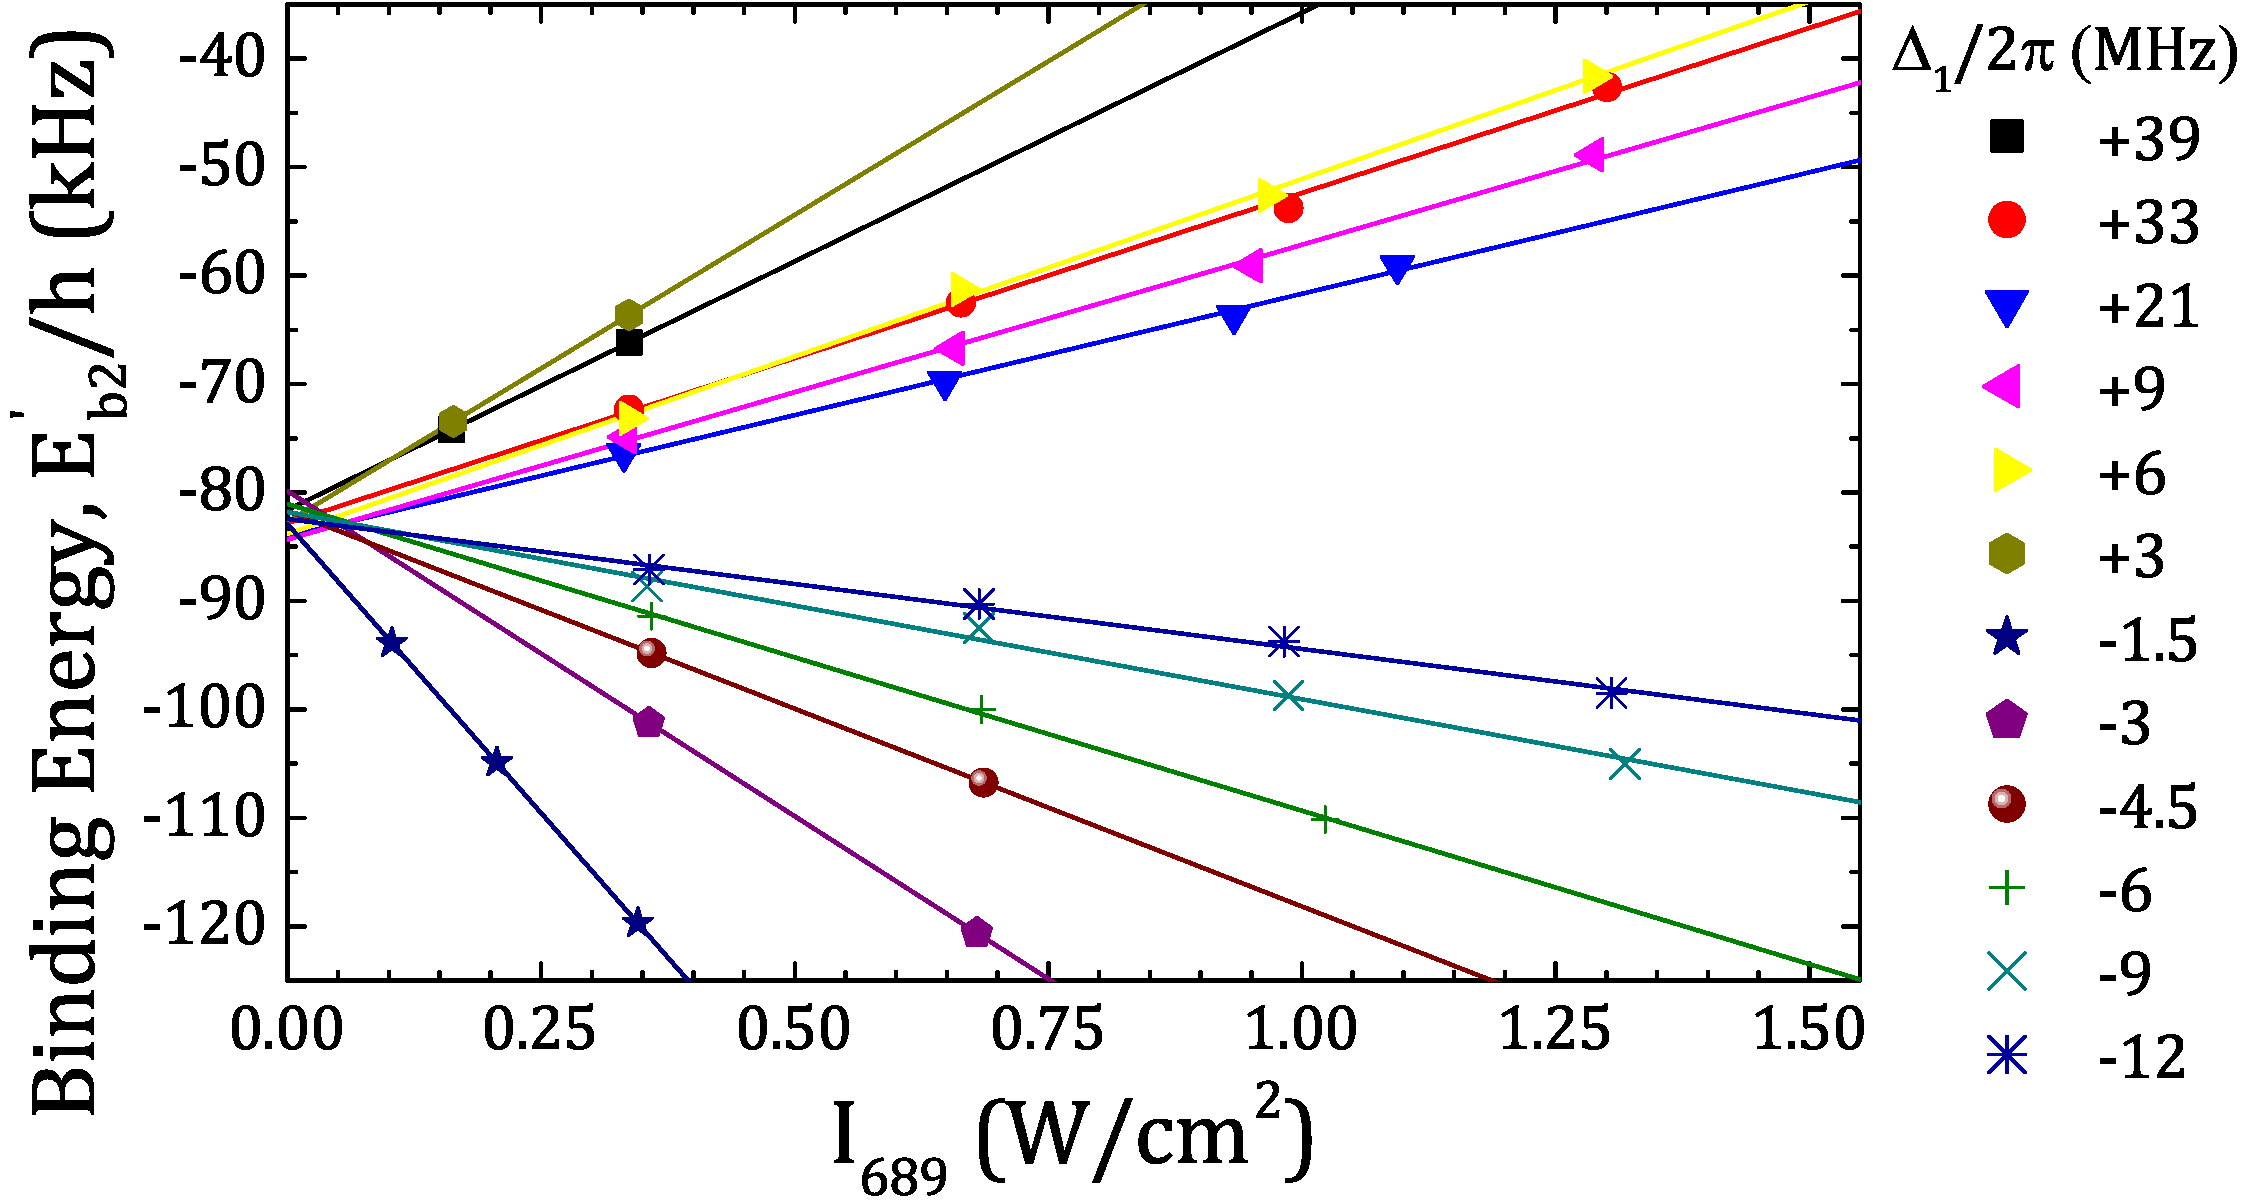
\includegraphics[width=\textwidth]{halo_susceptibility_vary_delta1.pdf}}
  \caption{Variation of halo susceptibility as a function of $\Delta_1$}{Two-photon PA resonance positions as a function of twice the single-beam excitation intensity, $2I=I_{689}$ for various intermediate state detunings, $\Delta_1$ .}
\end{figure}

Equation (\ref{Eq:BindingEnergyGao}) and the previous best value of the scattering length \cite{skt10} predict a binding energy of $E_{b2}=-86(3)$\,kHz. This agrees with our measurement, but by inverting Eq.\ (\ref{Eq:BindingEnergyGao}), we can use our increased accuracy in $E_{b2}$ to extract an improved value of the scattering length of $a=810.6(3)(9)$\,$a_0$, where uncertainties reflect statistical and systematic uncertainties in $E_{b2}$ respectively. The next higher-order term in $x_0={\bar{a}}/({a-\bar{a}})$ is likely to introduce a correction on the order of $100$\,Hz in Eq.\ (\ref{Eq:BindingEnergyGao}), creating a systematic uncertainty in $a$ that is about one third of the uncertainty from our measurement.

%Uncertainty in $C_6$ corresponds to an uncertainty of $\sim 15$\,Hz in the binding energy, and is negligible.

\section{Calculating the bound-bound Frank-Condon factor}
\label{sec:lowE_coupling}

%% paper
The proximity of $^{86}$Sr to a scattering resonance and the susceptibility of the halo binding energy to the intensity of the excitation light suggests  using light to tune the binding energy and scattering length as was done with optically assisted magnetic Feshbach resonances \cite{blv09,chx15}, which is closely related to the use of optical Feshbach resonances \cite{Fedichev1996a,Theis2004,Yamazaki2010,Blatt,Yan2013c}. Understanding the frequency-dependence of $\chi_{689}$ is important for investigating this possibility, so we extracted this parameter from spectra at a wide range of 689-nm laser intensities and detuning from the intermediate resonance ($\Delta_1$).

Figure \ref{Fig:ShiftsofLinesWithIntensity} shows
the resulting resonance positions, $E'_{b2}$, versus twice the single-beam intensity, $2I=I_{689}$. The shift in molecular binding energy is linear with intensity over the explored range, but varies greatly in magnitude and sign. From linear fits, we extract the AC Stark shift parameter $\chi_{689}(\Delta_1)$ through $E'_{b2}\equiv E_{b2}+h\chi_{689}(\Delta_{1}) I_{689}$ (Fig.\ \ref{Fig:ACStark}).

In the experiment, the total 689-nm intensity oscillates with 100\% contrast according to $I_{\text{total}}=I_1+I_2+2\sqrt{I_1I_2}\cos \left[(\omega_1-\omega_2)t \right]=2I\left\{1+\cos \left[(\omega_1-\omega_2)t \right]\right\}$. The functional form we use to fit the AC Stark shift reflects the time average of the intensity and neglects the interference term. To confirm that this is the correct description, we numerically solved the time-evolution for a three-level system with similar optical couplings and oscillating optical intensity as present during two-photon PA of a halo state. The Hamiltonian is
\begin{eqnarray}\label{Eq:ThreeLevelHamiltonian}
H=
\left(
    \begin{array}{ccc}
      0 & \Omega_{01}\left[\mathrm{cos}(\omega_1 t)+ \mathrm{cos}(\omega_2 t)\right] & 0 \\
      \Omega_{01}\left[\mathrm{cos}(\omega_1 t)+ \mathrm{cos}(\omega_2 t)\right] & E_{b1} & \Omega_{12}\left[\mathrm{cos}(\omega_1 t)+ \mathrm{cos}(\omega_2 t)\right] \\
      0 & \Omega_{12}\left[\mathrm{cos}(\omega_1 t)+ \mathrm{cos}(\omega_2 t)\right] & E_{b2} \\
    \end{array}
  \right)
\nonumber
\end{eqnarray}
For $\Omega_{01}\ll \Omega_{12} \ll |\Delta_{1}|\equiv |\omega_1-E_{b1}/\hbar|$, which is analogous to the experimental conditions used here, we find that the two-photon resonance is shifted by
\begin{equation}\label{Eq:ACStarkFullModel}
\frac{\hbar\Omega_{12}^{2}}{4\Delta_{1}}+\frac{\hbar\Omega_{12}^{2}}{4\left(\Delta_{1}-E_{b2}/h\right)}\approx
\frac{\hbar\Omega_{12}^{2}}{2\Delta_{1}}.
\end{equation}
This agrees with our observation of a shift that is linear with intensity, and implies that the susceptibility is related to the Rabi frequency for a single-beam intensity $I$ through $\chi_{689}\approx(\Omega_{12}/\sqrt{I})^2/(8\pi \Delta_1)$.



%follows $\delta={\Omega_{12}^{2}}/{2\Delta_{1}}$ in agreement with Eq. \ref{Eq:ACStarkFullModel}.
%If  a  single-resonance model, only describing coupling of the halo state $b_2$ to the intermediate state $b_1$, were accurate, then
%\begin{equation}\label{Eq:ACStarkFullModel}
%\chi_{689}\equiv \frac{\Omega_{2,12}^{2}}{8\pi\Delta_{1}}+\frac{\Omega_{1,12}^{2}}{8\pi\left(\Delta_{1}-E_{b2}\right)}
%\end{equation}
%We model the Stark shift  with a single resonance model,
%\begin{equation}\label{Eq:ACStarkFullModel}
% E'_{b2}\equiv E_{b2}+\frac{\hbar\Omega_{2,12}^{2}}{4\Delta_{1}}+\frac{\hbar\Omega_{1,12}^{2}}{4\left(\Delta_{1}-E_{b2}\right)}=
% E_{b2}+h\chi_{689}(\Delta_{1}) I_{689},
%\end{equation}
%where we have separated the contributions from the two beams, but for all data discussed here, both intensities are equal and $\Omega_{2,12}=\Omega_{1,12}$. The small difference in detunings of the two beams is shown but produces a negligible effect.

%It is important to note that the total 689-nm intensity oscillates with 100\% contrast according to
%$I_{total}=I_1+I_2+2\sqrt{I_1I_2}\cos \left[(\omega_1-\omega_2)t \right]=2I\left\{1+\cos \left[(\omega_1-\omega_2)t \right]\right\}$.
%Equation \ref{Eq:ACStarkFullModel} assumes assumes the AC Stark shift reflects the time average of the intensity and neglects the interference term. To confirm that this is the correct description, we numerically solved the time-evolution for a three-level system. The Hamiltonian is
%\begin{eqnarray}\label{Eq:ThreeLevelHamiltonian}
%H= \hspace{3in} \\
%\left(
%    \begin{array}{ccc}
%      0 & \Omega_{01}\left[\mathrm{cos}(\omega_1 t)+ \mathrm{cos}(\omega_2 t)\right] & 0 \\
%      . & E_{b1} & \Omega_{12}\left[\mathrm{cos}(\omega_1 t)+ \mathrm{cos}(\omega_2 t)\right] \\
%      . & . & E_{b2} \\
%    \end{array}
%  \right)
%\nonumber
%\end{eqnarray}
%For  $\Omega_{01}\ll \Omega_{12} \ll \Delta_{1}\equiv E_{b1}/\hbar-\omega_1$, which is analogous to the  coupling scheme for photoassociation, the shift of the two-photon resonance condition follows $\delta={\Omega_{12}^{2}}/{2\Delta_{1}}$ in agreement with Eq. \ref{Eq:ACStarkFullModel}.

This single-resonance model [Eq.\ (\ref{Eq:ACStarkFullModel})] describes the observed shifts well for detuning close to the $\nu=-2$ state of the $0^+_u$ molecular potential (small $\Delta_1$). For large positive $\Delta_1$, however, at which $\omega_1$ and $\omega_2$ approach atomic resonance, deviations indicate coupling to one or more other states (Fig.\ \ref{Fig:ACStark}). The most likely suspects are the $\nu=-1$, $J=1$ excited molecular state, bound by $1.633(1)$\,MHz, and the $^1S_0$+$^3P_1$ continuum. The sign of the deviation indicates that AC Stark shift of colliding $^1S_0$ atoms due to coupling to the $^3P_1$ state is dominant in this regime. We have neglected shifts due to collisions and the trapping laser, which are small at the large excitation-laser intensities used here.

\begin{figure} \label{Fig:ACStark}
\centerline{
  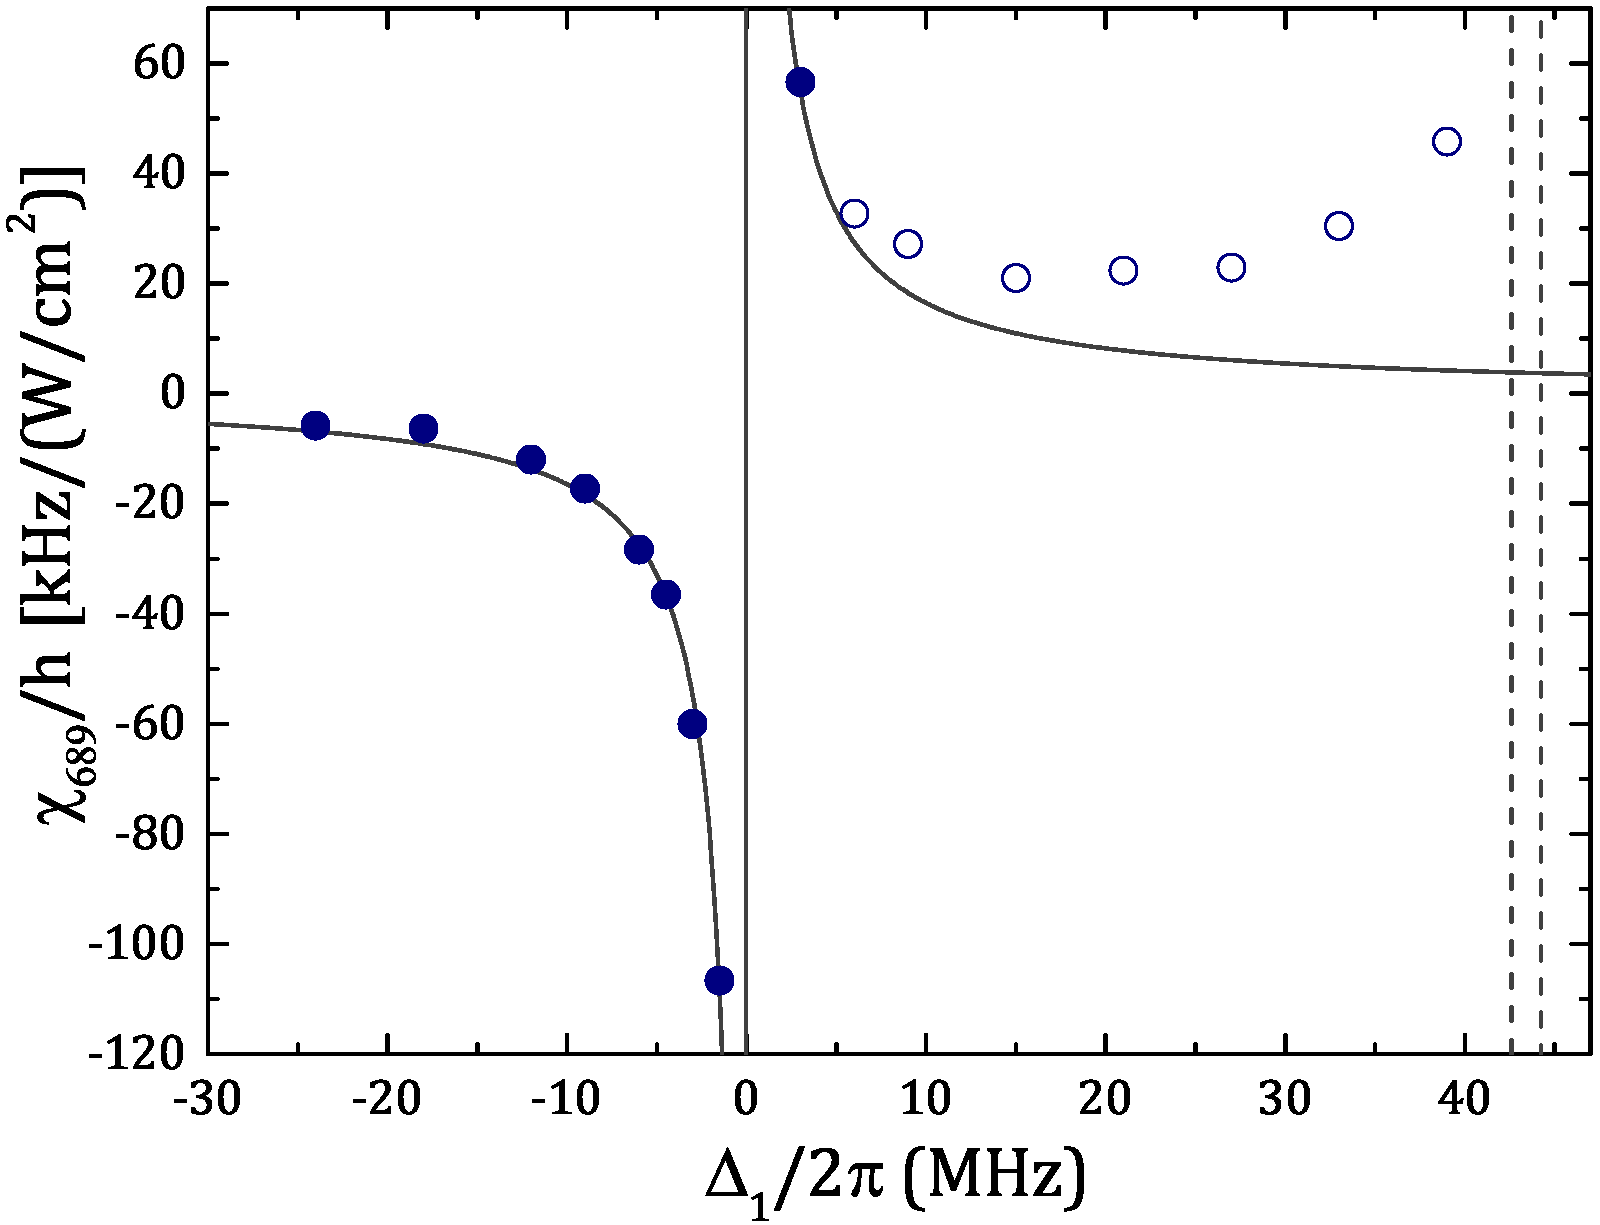
\includegraphics[width=\textwidth]{isolated_res_model.pdf}}
  \caption{Estimate of bound-bound coupling via isolated resonance model}{AC Stark shift susceptibility, $\chi_{689}$. Dashed lines indicate the positions of the $\nu=-1$, $J=1$ excited molecular state, bound by $1.633(1)$\,MHz, and the $^1S_0$+$^3P_1$ continuum. Solid and open symbols show experimental measurements of the susceptibility. Using only the solid symbols, we fit a single resonance model of the form $\chi_{689}\approx(\Omega_{12}/\sqrt{I})^2/(8\pi \Delta_1)$ and show this fit result as a solid line.}
\end{figure}

%(What is the AC Stark shift form the atomic transition on a single atom? The sign of the contribution from the unidentified state suggest that this is the main contribution as the red light approaches atomic resonances.
%
%Add in the figure just the contribution of the 1S0-3P1 atomic transition to the shift of the colliding atoms (2 x the single atom shift).)


%\begin{equation}\label{Eq:ACStarkFullModel}
% E'_{b2}\equiv E_{b2}+\frac{2\Omega_{12}^{2}}{4\Delta_{\nu=-2}}+
% \frac{2\Omega^{'2}}{4\Delta_{\nu=-1}},
%\end{equation}
%where $\Omega_{\alpha,b2}$ is the Rabi frequency for coupling between the halo state and state $\alpha$ of the $0^+_u$ molecular potential, and $\Delta_{\alpha}$ is the detuning of the 689 nm laser from resonance with the single-photon photoassociative transition to state $\alpha$.
%The factor of two before each Rabi frequency reflects %the fact that both excitation lasers contribute to the Stark shift with roughly equal detuning.

%We could not separately resolve the influence of coupling to the $^1S_0$+$^3P_1$ continuum, which is most likely also reflected in the $\Omega_{\nu=-1,b2}$ term, making the origin of this parameter not well defined.


A fit of the single-resonance model as shown in Fig.\ \ref{Fig:ACStark} yields $\Omega_{2,12}/2\pi\equiv\Omega_{12}/2\pi=800$\,kHz for $I=1$\,W/cm$^2$.
Note that $\Omega_{2,12}$ as defined here would be the splitting of the Autler-Townes doublet \cite{Pachomow2017a}, which differs from the Bohn-Julienne definition of the molecular Rabi coupling \cite{bju96}. From the measured $\Omega_{2,12}$, one can extract the Franck-Condon factor, $f_{\text{FCF}}$, reflecting the overlap of the ground and intermediate molecular states through
\begin{equation}\label{Eq:FranckCondonRabiFrequency}
	\Omega_{2,12}=\sqrt{f_{\text{ROT}}}\sqrt{f_{\text{FCF}}}\gamma_{\text{atomic}}\sqrt{\frac{I}{2 I_{\text{sat,atom}}}}
\end{equation}
where $I_{\text{sat,atom}}=2\pi^2\hbar c \gamma_{\text{atomic}}/(3\lambda^3)=3$\,$\mu$W/cm$^2$ is the atomic saturation intensity for the $^1S_0$-$^3P_1$ transition and $I=I_{689}/2$ is the single-beam intensity. The rotational factor $f_{\text{ROT}}$ accounts for the change in dipole moment from atom to molecule due to symmetry of the wave function and projection on a rotating molecular axis. Following the formalism described in \cite{Pachomow2017a}, $f_{\text{ROT}}=2$ for the $J=1\rightarrow 0$ bound-bound molecular transition studied here. This yields $f_{\text{FCF}}=0.03$.

%\textit{Why isn't there an AC Stark shift of the free-atom scattering state due to coupling to the excited molecular levels?
%}
%comment on loss for a given change...perhaps show large shift-data.

%\section{Higher-Order Raman Processes
%\label{sectionMultiphoton}}
%
%%For atoms, directed in the context of atom interferometry, as a coherent atomic beam splitter. First observation of Bragg scattering of atoms in a beam from a standing wave of light, including higher-order processes (up to 4th order - 9 photons mentioned) \cite{mom88}.(Absorption and stimulted emission of photons. Energy and momentum are conserved. Resonantly tuned so that atoms scatter mainly into one order. Kapitza-Dirac scattering had been observed previously.) Standing wave was fixed. Atoms came in with finite momentum that satisfied the Bragg condition for $\Delta E=0$.
%%
%%Careful study in similar experiments, observed up to 6th order \cite{gml95}.
%%Proposed in JETP paper \cite{dkc85}.
%%
%%With advent of essentially stationary atoms.increased control..Bragg spectroscopy from a moving standing wave starting with atoms in a BEC \cite{kdh99}
%
%At high laser intensities and for relatively small single-photon detuning ($|\Delta_1|\lesssim 5$\,MHz), we observe additional spectroscopic features
%%that appear to be peculiar to Raman spectroscopy of a halo state. A
%as shown in Fig.\ \ref{Fig:multiphotondata}. For single-beam intensity $I$, the main feature appears at $\omega_1-\omega_2=E'_{b2}(I)/\hbar$, where $E'_{b2}(I)$ is shifted predominantly by the AC Stark shift from the excitation light, and
%additional features appear at
%subharmonics, $\omega_1-\omega_2=E'_{b2}(I)/n\hbar$ for $n=2,3..$ up to as high as $n=5$. The frequency pattern and the ratios of signal strengths suggest that the additional lines correspond to higher-order multi-photon Raman processes as shown in Fig.\ \ref{Fig:multiphotonschematic}, with the $n^{th}$ process involving $2n$ photons. A large negative AC Stark shift $\Delta_1<0$ %(Sec.\ \ref{sectionACStark})
%facilitates observation of this phenomena because it increases the binding energy of the halo state, stretching the frequency spectrum and making room for resolved subharmonics.
%
%In theoretical descriptions of photoassociation of colliding, ground-state atoms to weakly bound molecular levels on the ground-state potential, process of higher order than two-photon ($n=1$) were not considered \cite{bju96,bju99}.
%To our knowledge, they have never been observed before now.
%%The similarity to a higher-order Bragg process might explain why this phenomena has not been seen before and highlights an unusual feature of photoassociation to a halo state.
%The extremely small binding energy associated with the halo state creates much more favorable conditions for observing this phenomena, however. It results in small intermediate detunings ($\sim E'_{b2}(I)/\hbar$), maintaining a high effective Rabi frequency for the multi-order process.
%
%There are similarities to other well-know spectroscopic phenomena. For example, non-linear Raman processes are commonly used in analytic chemistry, but  typically involves more, near-resonant laser fields \cite{bor82} rather than just two as in our situation. Higher order Bragg spectroscopy of atoms, which can be viewed as a multi-order Raman process driven by two light fields, is perhaps more similar. This was developed in the context of atomic beams for atom interferometry \cite{dkc85,mom88,gml95} and later applied to utlracold samples \cite{kdr96,kdh99,sic99}. An important difference however, is that in Bragg spectroscopy, lasers are aligned for momentum transfer from the light fields to the atoms, making the resonance condition sensitive to initial atom momentum.
%
%
%
%To check whether our interpretation of higher-order processes is correct, we simulated the spectrum using a three-level lambda system connected by two coherent light fields, as shown in Fig.\ \ref{Fig:ThreelevelSystem}. This also
%will investigate whether the process depends on the fact that this is a scattering problem, involving an initial state of two free atoms.
%To model the loss, we assign loss rates of $\gamma_1=2\gamma_{atomic}$ to state $1$ and $\gamma_2=xx$,Hz to $2$ reflecting the broadening of the PAS line discussed in Sec.\ \ref{xx}. It is important to note that the Hamiltonian governing the system retains both laser fields in the coupling between states $0$ and $1$ and between $1$ and $2$. This is necessary because the frequencies of both laser fields are so similar, or, equivalently, the $0-2$ energy difference is so small. The $1-2$ coupling is set to the value determined from the observed AC Stark shift (Sec.\ \ref{sectionACStark}). The $0-1$ coupling is not well determined from the experiment, and it actually does not have a rigorous analog because the Hamiltonian doesn't reflect that state $0$ is a two-body scattering state. We simply use $\chi\ll 1$ as a fit parameter. Nonetheless, this simple approach captures the high-intensity spectrum extremely well.
%We find $\chi\ll 1$, showing the
%$1-2$ coupling is much stronger than the $0-1$ coupling, as observed in the experiment.
%


%% %% %% %% %% %% %% %% %% %% %% %% %% %% %% %% %% %% %% %% %% %% %% %% %% %% %% %% %% %% %% %% %% %% %% %% %% %% %% %% %% %% %% %% %% %% %% %% 
%% other thoughts
From the formula for the line shape we can see that it depends on the spatial distribution of the atoms. The standard approximation made when measuring these types of systems is to ensure loss does not cause heating of the atoms during photoassociation. Heating results in re-equilibration of the atomic density distribition, which in turn effects the rate of loss creation. Without independent controls to keep the system in thermal (and therefore spatial density) equlibrium.

What are the things the rate equation deals with?

We need the desnity distribution.

In a harmonic trap, there if a simp[le anayltic form to the density distribution of a thermal gas. From Mi's work (and others) we know that this is only an approximation that is valid when eta is approx greater than 4. When greater than 4 we can apply the high-eta approx and the trap frequencies along a particular direction reduce to <eq>.

However, the trap we did this experiment in were at eta's of 1 or less so we don't have an analytic solution to the spatial distribution. Since this could be a problem we need to know what the trap looks like.

We measure trap oscillation freq. at several different powers and model the trap using the utility outlined somewhere else.

From the numeric model, we can define a spatially depedent eta which is determined by the local trap depth which is simply the difference between the local potential energy and the global depth. This is illustrated in fig something.

The spatial information is not only important for the density determination, but also for the range of available thermal energies. Consider two atoms near the local bottom of the trap. By definition, in equilibrium, a single atom may only have up to the trap depths worth of energy since any additional energy would result in its expulsion from the trap. In this case, in a relative momentum frame, the allowed collision energies range from zero to two times the trap depth. Similarly, as we move towards the edge of the trap the range of accessible collision energies shrinks. This additional weighting factor may be viewed as having a local truncasted Boltzmann ditribution at every point in space. 

Normally the BZ dist goes to infinity but here we have a cutoff at 2 trap depeth. The most naive approx would be to simply consider the BZ and harshly truncate at 2 trap depth. We tried this

We know this is unphysical since we should expect that the probability of observing a certain momenta at a certain point in space, should smoothly tend zero towards as we approach the edge of the trap. To see what this looks like we (and determine how important the effect is) we rederive the relative momentum distribution.

<Some stuff about center of mass and relative>

What were all the cases and conclusions of having done this? Remember to consider what the different cases are. If the total relative energy can be X then how does that get split up? Use the plots to show this limiting behavior. Like if particle 1 has all the energy then there is only one possible value for particle 2 (and vice versa).


DERIVATION for truncated trap below

Need to lookup references for this molecular chaos assumption. What about egodicity? How to discuss that we may not be completely ergodic?

What does my potential look like? Can I make it a piecewise function? How should I introduce this part?

Where does the f equation come from? I believe this is just the normalized boltzmann factor for probability to occupy a particlar state.

\noindent
We can truncate this single particle distribution by 
\begin{equation}
\label{eq:trun_single_particle_prob}
		 f_{ \vec{r} }( \vec{p} ) = A \left(\frac{1}{2 \pi k_B T}\right)^{3/2} e^{\left(\frac{-p^2}{2 m k_B T}\right)} \Theta \left( \epsilon_{max} - U( \vec{r} ) - \frac{p^2}{2 m} \right)
\end{equation}

\noindent
where A is a normalization constant which ensures $\int_0^\infty f_{ \vec{r} }( \vec{p} )\,d \vec{p} = 1 $ and $\Theta(x)$ is the Heaviside function defined by

\begin{equation}
\label{eq:heaviside}
	\Theta(x)=
	\begin{cases}
		1 &\text{if } x \geq 0, \\
		0 &\text{if } x < 0
	\end{cases}
\end{equation}

We got a certain answer with the way shown in the paper.

We can also use a completely different method that ignores all the consdierations of the last few sections. As was done in the calcium paper, we could simply fit the blue edge of the feature using a model function which can capture the high level features of the lineshape. Get the same answer. SHOW PLOTS TO THIS AFFECT AND COMPARE



Maybe go a little into the isolated resonance model (or at least recall), then tie into how we can measure the susceptibility across several different detunings which can give us the coupling to intermediate level. The first order analysis of this data suggest a bound-bound rabi freuqnecy of \hl{BLAH}. 

Point out the curling up at the end and say how the simple isolated resonacne model cannot predict. A full coupled channel calculation probably could but in the spirit of the Bohn and Julienne semi-classical approach, we set out to derive an approximate analytic expression to determine the binding energies. THis is presented in the next chapter.








Lastly, we note that in the context of photoassociation, the center-of-mass component of Eq.\ref{eq:two_particle_prob_inf_atomFrame} is not typically considered as typical PAS experiments are performed utilizing broad dipole allowed transitions which have linewidhts much greater than the doppler width thus only the relative momentum between particles is important for determining the loss rate coefficeint K discussed in \hl(somewhere). 



The case of PA using narrow intercombination line transitions found in alkaline-earth-metal atoms 


In general K is considered as a boltzmann average over a single loss rate constant
This can be seen in \cite{Ciuryo2004} Eq. 1 where the loss rate constant is given by

\begin{equation}
\begin{split}
\label{eq:ciuryo04_eq1}
		 K(\Delta,T) &= \left\langle\mathcal{K}(\Delta,\vec{P}_c,\vec{p}_r)\right\rangle \\
		 &= \int d^3\vec{P}_c \; f_M(\vec{P}_c) \int d^3\vec{p}_r \; f_{\mu}(\vec{p}_r) \; \mathcal{K}(\Delta,\vec{P}_c,\vec{p}_r)
\end{split}
\end{equation}



To this end we can integrate out the center of mass component to obtain the distribution most typically relevant to photoassociation.

By the time I've gotten to this I have already introduced K and that is not what I wanted to do. 

conclusion
here is the modified version of K we need for a trap that has a truncated energy disttribution

to get there
normal version of K is \hl{given in ch3}
this K can be given in terms of f? 
this ver4sion of f is given in the appendix
	why do I integrate out the com component?




typical PAS experiments utilize dipole allowed transitions which have linewidths many times larger than the 



We now perform a change of variables using Eq. and Eq.\ref{eq:two_particle_prob} can be rewritten as 




Need to make a connection between dipole matrix element, wigner threshold, and infinite squarer step potential. This infiinite square step can be viewed as a dilute ideal gas. 

To prove this assumption I want to show that using the square step I can get the same equations like in Eq. 1 of the 99 paper. Then once we know the infinite energy behavior (valid for only a particular portion of energy due to s-wave constraint) then we can ask what happens if f(p) is truncated. 

In the s-wave limit I need to write K as a function of f(p) (should do this in the appendix proof and reference in body). Given the form of the loss rate constant K, our problem reduces to determining the form of f(p) when eta is finite.

Ok, so need to reference \cite{Ciuryo2004} to motivate usage of center of mass. Then use \cite{Nicholson2015a} Eq. 43 to reference the particular form 


what is the throughline I want to make? Develop K$_{in}$ $\rightarrow$ recast in terms of P distribution $\rightarrow$ show how we can replace the normal dist with a truncated dist $\rightarrow$ explore the effects of that truncation 